\documentclass[10pt,a4paper]{article}
\usepackage[utf8]{inputenc}
\usepackage[T1]{fontenc}
\usepackage{lmodern}
\usepackage[margin=2.2cm]{geometry}
\usepackage{amsmath,amssymb,amsthm,mathtools}
\usepackage{booktabs,array,tabularx,multirow,longtable}
\usepackage{graphicx}
\usepackage{xcolor}
\usepackage{enumitem}
\usepackage[hidelinks]{hyperref}
\usepackage[numbers,sort&compress]{natbib}
\usepackage{tikz}
\usetikzlibrary{positioning,arrows.meta,calc,fit}

\setlist{nosep,leftmargin=1.4em}
\setlength{\parskip}{2pt}
\newtheorem{proposition}{Proposition}
\newtheorem{corollary}[proposition]{Corollary}
\bibliographystyle{plainnat}

% Evidence classes (programme standard): every number carries one.
\newcommand{\ev}[1]{{\scriptsize\textsuperscript{\textcolor{gray}{[#1]}}}}
\newcommand{\evM}{\ev{M}}   % MEASURED by us, artifact in the repository
\newcommand{\evP}{\ev{P}}   % PUBLISHED, cited
\newcommand{\evI}{\ev{I}}   % INHERITED from a programme document, not re-verified
\newcommand{\evE}{\ev{E}}   % ESTIMATED (closed-form arithmetic, no timing)
\newcommand{\evH}{\ev{H}}   % HYPOTHESIS, to be tested
\newcommand{\cell}[1]{\texttt{#1}}
\newcommand{\Real}{\mathbb R}

\title{\textbf{HiCAP: Hierarchical Contrastive Action Priors on a Frozen Vision--Language Backbone\\
for Elastic, Imagination-Aware Driving}}
\author{TanitAD programme \\ \small Design and pre-registration paper \\ \small (working draft, 2026-09-29)}
\date{}

\begin{document}
\maketitle

\begin{abstract}\noindent
Autonomous-driving policies built on vision--language models (VLMs) inherit world knowledge but decode actions
one token at a time, which is bound by memory bandwidth on an in-vehicle computer. Contrastive selectors (CLM, CoVer-VLA)
replace generation by a single prefill pass and a similarity search over cached action embeddings, but they treat the action set
as flat and small, inherit the marginal-frequency bias of their loss, and neither predict outcomes nor budget their sensors.
We describe \emph{HiCAP}, a design that keeps what made CLM work---a frozen backbone, two small trainable heads, cached action
embeddings, a calibrated cosine score, a staged curriculum---and adapts it to driving. (i)~The action side is a \emph{tree}
built from the programme's frozen tactical and strategic token vocabulary, refined by a two-stage code over
kinematic-prior residuals, so that vocabularies of $10^{5}$--$10^{7}$ leaves are searched by beam retrieval
(a cost proposition and a measured pruning study are given). (ii)~A short chain of prior-encoded rules---kinematic
feasibility, state-conditioned admissibility, hysteresis, and conformal keep-sets with a stated recall bound---reduces the candidate set
before any expensive computation, and the survivors are fed back to the backbone for candidate-conditioned re-scoring.
(iii)~We show that the InfoNCE optimum is a pointwise mutual information whose argmax is biased under a cruise-dominated prior and
correct it with a fitted log-prior. (iv)~Imagination is restricted to an \emph{identifiable} factorisation---a non-reactive scene
forecast, a known kinematic map and a contrastive future critic---gated by two-head agreement.
(v)~An elastic-sensing controller chooses cameras and visual-token budgets per tick from cheap cues, and an audio branch is tokenised
into the backbone's embedding space with explicit controls. (vi)~A frozen multi-billion-parameter backbone violates the programme's
sub-300\,M target, so the interface is a fixed-dimension embedding space that a distilled student can occupy, with a decision-preservation
bound. We report only what exists: closed-form propositions with proofs, a real-data check that a physical-limit mask
removes $78\%$ of a trajectory set while retaining all $881/881$ logged futures, toy measurements of the prior bias, and a pre-registered
protocol with both outcomes committed for every hypothesis. No end-to-end HiCAP model has been trained.
\end{abstract}

% ---------------------------------------------------------------------------
\section{Introduction}\label{sec:intro}
% ---------------------------------------------------------------------------
A driving policy has to do three things that pull in different directions: know a great deal about the world (what a school bus
implies, what a siren means), reason at several time scales (which road to take, which manoeuvre to start, how to move the
wheel now), and fit into a fixed power and latency envelope. Large vision--language models supply the first; the field's dominant
way of using them, autoregressive generation of a plan or trajectory \citep{hwang2024emma,renz2025simlingo,nvidia2025alpamayor1},
works against the third, because decoding one token requires streaming the model's weights once and is bound by memory bandwidth rather than arithmetic on an edge SoC.

\emph{Contrastive Language Models} (CLM) showed a different way to use a large frozen model \citep{kwok2026clm}: read the model
once (prefill), map the last hidden state and each candidate action through two small MLP heads into one shared 512-dimensional
space, and choose the action with the highest cosine score. Action embeddings are computed once and cached, the backbone is never
updated, and a three-stage curriculum trains the heads on cached features. CoVer-VLA transferred the recipe to robot manipulation with
a frozen image encoder and numeric action chunks \citep{kwok2026cover}. Both treat the action set as a flat list.

Driving has structure that a flat list wastes. Actions are \emph{hierarchical}: a route-level intent, a manoeuvre (lateral and
longitudinal, chosen separately), and a continuous trajectory. Actions are \emph{highly prior-structured}: physics, the current
speed, the last plan and the navigation command exclude most of the space before any learning. The candidate set can be very large
if it can be searched cheaply. And the input side is not fixed: not every camera or token is worth its cost at every instant, and some
decisive cues (a siren) are not visual at all.

\paragraph{Programme context.}
HiCAP is the vision--language arm of TanitAD, a programme building sub-300\,M hierarchical latent world models for driving.
The programme's newest reference planner line (anchored diffusion, REF-C) exposes the problem this paper addresses. On the parity
lineage, the best candidate in a 256-anchor fan has an ADE@2\,s of $0.1640$\,m while the candidate the planner selects has
$0.4714$\,m\evI~(REF-C-XL, 40 validation episodes; registry \S4). On the newest lineage, trained on the v7 corpus, the
hold-the-current-action control scores $0.2996$\,m and the pre-registered constant-velocity-extended control $0.2874$\,m, against $0.2975$\,m and $0.3079$\,m
for the two best trained arms\evI~(registry \S4.6--4.8; 4{,}823 windows, 141 episodes, none separated from the controls); the deficit lies
on the longitudinal axis, which carries $92.2\%$ of the gap between the planner and the hold control\evI. Strategic (route-level) quality
is reported UNAVAILABLE for two of those arms and $0.7708$ route accuracy against a $0.6742$ majority rate for the third\evI. In short, the
programme's bottleneck is neither the candidate set nor the lateral path; it is the \emph{decision}, especially the longitudinal one, and it is
under-supervised at the tactical and strategic levels. HiCAP is our attempt to build the decision maker properly on a backbone that already
knows the world.

\paragraph{Contributions.} We (1)~define a hierarchical action tree from the programme's frozen tactical/strategic token vocabulary with a factored path-by-profile trajectory vocabulary beneath it, with a retrieval-cost proposition, a beam-miss bound and a real-data pruning study (\S\ref{sec:vocab}, \S\ref{sec:theory}, \S\ref{sec:prelim});
(2)~show that a CLM-style contrastive selector is prior-biased and give a corrected, per-level objective (\S\ref{sec:train}, Corollary~\ref{cor:bias});
(3)~specify prior-encoded pruning with a conformal recall bound and a candidate-conditioned re-scoring stage that returns survivors to the backbone (\S\ref{sec:prune});
(4)~restrict imagination to what data can identify, in three tiers (soft outcome-aware targets, an analytic forecast of exogenous descriptors, a gated critic with a disagreement veto) and show in a toy that most apparent gain is target shape (\S\ref{sec:imag}, Proposition~\ref{prop:ident});
(5)~add elastic sensing (cameras, tokens, embedding width) and an audio branch tokenised into the backbone's space (\S\ref{sec:elastic});
(6)~separate a frozen reference model from a distilled sub-300\,M student with a decision-preservation guarantee (\S\ref{sec:eff}, Proposition~\ref{prop:distill});
and (7)~commit a pre-registered protocol, including negative controls and both outcomes for each hypothesis (\S\ref{sec:protocol}).

\paragraph{Scope and evidence convention.}
This is a design and pre-registration paper. \textbf{No HiCAP model has been trained.} Everything quantitative is one of: a closed-form
statement with a proof; a measurement on committed data using only inference-time quantities; a toy simulation; arithmetic; or a number
inherited from a programme document. Each number carries an evidence tag: \evM{} measured by us with an artifact in the repository,
\evP{} published and cited, \evI{} inherited from a programme document and not re-verified here, \evE{} closed-form estimate (no timing),
\evH{} hypothesis. Where two programme documents disagree, the model registry is the tie-breaker and the conflict is reported (\S\ref{sec:limits}).

% ---------------------------------------------------------------------------
\section{State of the art}\label{sec:related}
% ---------------------------------------------------------------------------
\paragraph{Planning heads: from regression to scored candidate sets.}
End-to-end driving moved from single-trajectory regression \citep{hu2023uniad,jiang2023vad} to multimodal heads
(anchored diffusion in DiffusionDrive \citep{liao2024diffusiondrive}) and to \emph{scoring} a fixed or generated candidate set.
VADv2 scores a vocabulary of 4{,}096 trajectories with a learned probability \citep{chen2024vadv2}; Hydra-MDP distils
rule-based metric teachers into a per-candidate scorer over an 8{,}192-entry vocabulary and reports that per-family
sub-scores beat one scalar \citep{li2024hydramdp}; GTRS and DriveSuprim score dense vocabularies coarse-to-fine
\citep{li2025gtrs,yao2025drivesuprim}; WoTE scores candidates with a BEV world model \citep{li2025wote};
ZTRS learns the scorer from reward alone \citep{li2025ztrs}; GoalFlow conditions generation on a goal point \citep{xing2025goalflow}.
The shared lesson is that separating \emph{what can be proposed} from \emph{what is chosen} pays, and that the gap between the two is
large. In our own reference planner (an anchored-diffusion arm, REF-C, parity lineage, 40 validation episodes) the best candidate in a 256-anchor fan has an ADE@2\,s of $0.1640$\,m while the candidate it selects has
$0.4714$\,m\evI{} (registry \S4; introduction), so the gap between proposing and choosing is larger than the gap between planners. None of these systems is hierarchical, cacheable, or elastic in its sensing.

\paragraph{Vision--language(--action) driving.}
EMMA \citep{hwang2024emma}, DriveVLM \citep{tian2024drivevlm}, SimLingo \citep{renz2025simlingo} and Alpamayo-R1
\citep{nvidia2025alpamayor1} decode trajectories or actions autoregressively from a VLM, often with reasoning traces;
DriveVLM-Dual and FASIONAD pair a slow reasoner with a fast planner \citep{tian2024drivevlm,qian2024fasionad}.
Autoregressive decode is memory-bandwidth-bound on an edge SoC, which is the regime a vehicle computer lives in
(\S\ref{sec:eff}). HiCAP keeps the VLM's world knowledge but replaces generation by a single prefill pass and a
retrieval over cached action embeddings.

\paragraph{Contrastive and energy-based decision models.}
Contrastive Language Models (CLM) freeze a language model, train two small projection heads with bidirectional InfoNCE
on cached embeddings, and choose the action whose embedding best matches the state; action embeddings are cached, and as a best-of-$N$ verifier the
model reaches 81.6\% on DeepSWE and 87.6\% on Terminal-Bench~2.1 at 4.1--5.7$\times$ lower latency than a generative verifier
\citep{kwok2026clm}. Its closest robotics relative is CoVer-VLA, a frozen SigLIP~2 with attention pooling over patch tokens, a numeric
action-chunk tower and symmetric InfoNCE that verifies VLA action candidates \citep{kwok2026cover}. Earlier, Implicit Behavioural
Cloning used an InfoNCE energy over sampled counter-examples \citep{florence2021ibc}, later out-performed by diffusion
policies \citep{chi2023diffusionpolicy}, and VINN retrieves nearest-neighbour actions \citep{pari2021vinn}. Contrastive RL
interprets the critic as a discounted future-state occupancy \citep{eysenbach2022contrastiverl,wang2025thousandlayer}.
On the theory side the InfoNCE optimum is a pointwise mutual information \citep{oord2018cpc,poole2019variational},
the long-tail prior is removed by logit adjustment \citep{menon2021logit}, and dot-product retrieval has
provable dimensionality limits \citep{weller2025limits} that motivate late-interaction re-ranking \citep{khattab2020colbert}.
Prior contrastive selectors treat the action set as flat, text or a small numeric chunk, and none imposes a prior over a hierarchical vocabulary, predicts outcomes in the shared
space, or budgets its sensors.

\paragraph{Latent world models and imagination.}
Latent prediction on top of frozen or self-supervised encoders (V-JEPA~2 and its action-conditioned variant
\citep{assran2025vjepa2}, DINO-WM \citep{zhou2024dinowm}, Dreamer~4 \citep{hafner2025dreamer4}) supports planning without
pixel decoding, and world modelling as dense supervision amplifies data scaling for driving VLAs \citep{li2025drivevlaw0}.
Anti-collapse without heuristics is provided by sketched isotropic regularisation \citep{balestriero2025lejepa}. Our own programme
measured two failure modes that this literature does not foreground: a world model that faithfully rolls out an implausible
candidate (consistency is not plausibility) and imagination confidence that rises as rollout fidelity decays. HiCAP therefore restricts
imagination to an identifiable, non-reactive scene forecast plus a known kinematic map (Proposition~\ref{prop:ident}).

\paragraph{Elastic sensing, token budgets, and audio.}
Token merging and pruning reduce visual tokens at small accuracy cost \citep{bolya2023tome,chen2024fastv}; Matryoshka
representations make one embedding usable at several dimensions \citep{kusupati2022matryoshka}.
Multi-camera driving VLMs fix a camera set; we instead \emph{choose} the set per tick. Audio enters language models either through a frozen speech encoder and projector
\citep{radford2022whisper} or natively in omni-modal models; joint audio--visual embedding spaces are studied in
\citep{girdhar2023imagebind}. Driving-relevant sounds (sirens, horns) are absent from standard driving corpora, so
the audio path must be built and controlled differently (\S\ref{sec:audio}).

\paragraph{Safety layers.}
Runtime assurance around a learned planner uses control barrier functions \citep{xiao2023barriernet} and distribution-free coverage
sets \citep{angelopoulos2021gentle}; HiCAP's candidate set is a natural place to apply both before selection.

% ---------------------------------------------------------------------------
\section{Problem setting and data interface}\label{sec:prelim-setting}\label{sec:problem}
% ---------------------------------------------------------------------------
\paragraph{Decision problem.}
At each tick $t$ the system receives a state $s_t=(I_t^{\mathcal S_t},\,e_t,\,n_t,\,u_t)$: frames $I_t^{\mathcal S_t}$ from a chosen
camera subset $\mathcal S_t$ (three frames, 100\,ms apart, per camera); the ego kinematic state $e_t=(v,a_{\text{lon}},\dot\psi,\kappa)$ at the
cycle time; a navigation command $n_t\in\{\text{follow},\text{left},\text{right}\}$ with optional range and time arguments; and, in the audio arm only,
a window of microphone samples $u_t$. It outputs a 6\,s ego trajectory $\hat y\in\Real^{8\times2}$ at the slots
$t_k\in\{0.5,1,1.5,2,3,4,5,6\}$\,s in the ego frame, which is the trajectory contract of the programme's planner line.
The decision is a \emph{leaf} $a=(v_1,v_2,v_3)$ of the action tree of \S\ref{sec:vocab} plus a small continuous refinement $\delta\in\Real^{8\times 2}$:
$\hat y=\pi_{\text{prior}}(e_t)+\rho(v_3)+\delta$, where $\pi_{\text{prior}}$ is a constant-turn-rate-and-acceleration (CTRA) roll-out of the ego state and
$\rho(v_3)$ is the residual profile of the leaf's code.

\paragraph{Data.}
We build on the newest programme corpus, not on the older parity corpus that the repository's default branch still describes.
The corpus is the private Hugging Face dataset \texttt{tanitad-v7-training-corpus}: $4{,}719$ clips, $26.2$ hours of front-camera driving,
$4{,}572$ train and $147$ evaluation clips, corpus id \texttt{a48251e89c7a8603}, label schema \texttt{s2-geom-v7}, released as v7, v7.1, v7.2 and v8.1
(the vocabulary is identical across releases; releases add fields)\evI. It is deliberately a \emph{new comparability domain}: it does not re-select
the canonical parity corpus of $2{,}376$ episodes, and arms trained on it are compared only with arms trained on it. Frames are a cylindrical
projection at $256\times640$ pixels covering a true $120^\circ$ field of view (linear in azimuth, $f_{\text{ref}}=305.577$), with a mandatory
per-clip vertical crop because two camera rigs differ by about $215$ pixels. Only the front-wide camera is cached; the upstream dataset has seven
cameras, which matters for \S\ref{sec:elastic}. No corpus the programme uses carries audio\evM{} (36 upstream features, none audio; the shipped mp4 audio track
is unprobed).

\paragraph{What the labels are, and what they are not.}
Labels may use privileged quantities (ego future, other agents); inference may not. Table~\ref{tab:inputs} states, for every quantity,
whether it is a training label, an admissible inference input, or an evaluation stratifier only. The strategic and tactical tokens are derived offline from the
\emph{ego's own future path} (geometry), so they are legitimate targets and inadmissible inputs. The perception-style tactical goals
(traffic-light colours, gap targets, oncoming reactions) are teacher signals parsed from Alpamayo's chain-of-causation text; $49.6\%$ of records carry at least one
goal marked disputed and traffic-light colour was never independently verified\evI. They may supervise auxiliary heads but never enter as inputs, and every head on them
carries an ego-only control.

\begin{table}[t]
\centering\footnotesize
\caption{Admissibility of each quantity. \emph{Label} = offline supervision (privileged signals allowed). \emph{Input} = available at inference.
\emph{Strat.} = evaluation stratifier only. The navigation command is an oracle input by construction (it is the ego's own future turn), admitted under
a programme ruling as a first-class route signal and stamped as such in every run; the nav-zero and nav-shuffled controls quantify what it buys.}
\label{tab:inputs}
\begin{tabular}{@{}p{4.6cm}p{2.5cm}p{2.7cm}p{5.0cm}@{}}
\toprule
quantity & source & role & note \\ \midrule
frames (front-wide, 3$\times$100\,ms; further cameras when cached) & sensor & Input & cylindrical $256\times640$, per-clip crop \\
ego state $e_t$: $v,a_{\text{lon}},\dot\psi,\kappa$ at cycle time & sensor/CAN & Input & legal initial state; dropout with a learned null row \\
navigation command $n_t$ & ego-future & Input (stamped oracle) & controls: nav-zero, nav-shuffled \\
audio window $u_t$ & microphone & Input (audio arm) & needs an explicit ruling; no corpus \\
strategic tokens $g_{\text{str}},a_{\text{str}}$ & ego-future geometry & Label & band $[8,30]$\,s; four goals and two actions empty \\
tactical actions $a_{\text{tac}}^{\text{lat}},a_{\text{tac}}^{\text{lon}}$ & ego-future geometry & Label & band $[2,6]$\,s; factored, never flattened \\
tactical goals $g_{\text{tac}}$ (22, multi-label) & geometry + Alpamayo text & Label (aux) & 22 exclusive pairs; eight goals with $n<30$ \\
goal point $g_{\text{tac}}.\text{anchor}$ & ego-future & Label & predicted, never supplied \\
3-D agent tracks & \texttt{obstacle.offline} join & Label (cost heads) & $96.83\%$ of train clips \\
\texttt{tac\_SIT}, \texttt{disputed}, \texttt{alpamayo.*} & Alpamayo text & Strat. only & never an input \\
\texttt{nav\_30s}, \texttt{speed\_max\_input} & ego-future & Label / oracle & not built into any arm here (echo of the ego's realised speed) \\
situation-classifier output & --- & \textbf{absent} & HiCAP has none; goal path stays disjoint from it \\
\bottomrule
\end{tabular}
\end{table}

\paragraph{Information-disjointness of the goal path.}
Two programme rules bind the design. First, a route or goal input may not carry the output of a situation classifier, otherwise attribution between
goal and classifier is lost and the classifier is scored through the planner. HiCAP contains no situation classifier; its only route-side input is the
stamped navigation command, and evaluation-time situation strata (\texttt{tac\_SIT}) never re-enter. Second, the parent's selection restricts the child candidates
(a hard beam) but is not fed to the child's state readout, so the child level cannot echo the parent's decision as a feature; the control ``flat tactical'' (no parent restriction)
tests whether the restriction itself matters (\S\ref{sec:protocol}).

% ---------------------------------------------------------------------------
\section{Method}\label{sec:method}
% ---------------------------------------------------------------------------
Figure~\ref{fig:arch} shows the system. A frozen VLM turns camera frames into semantic tokens at a slow rate; a tiny trainable
motion adapter supplies what a frozen single-frame model cannot; a small fusion transformer with three level queries produces one unit-norm
state readout per decision level; and the action side is a tree of cached embeddings searched top-down under a chain of prior-encoded
pruning rules. Language never generates anything: the language tower embeds token definitions once, and is used at run time only by the
optional System-2 verifier (\S\ref{sec:prune}).

\begin{figure}[p]
\centering
\resizebox{\textwidth}{!}{% Architecture overview of HiCAP (TikZ), vertical flow, fixed grid (1 unit = 1 cm), natural width ~18 cm.
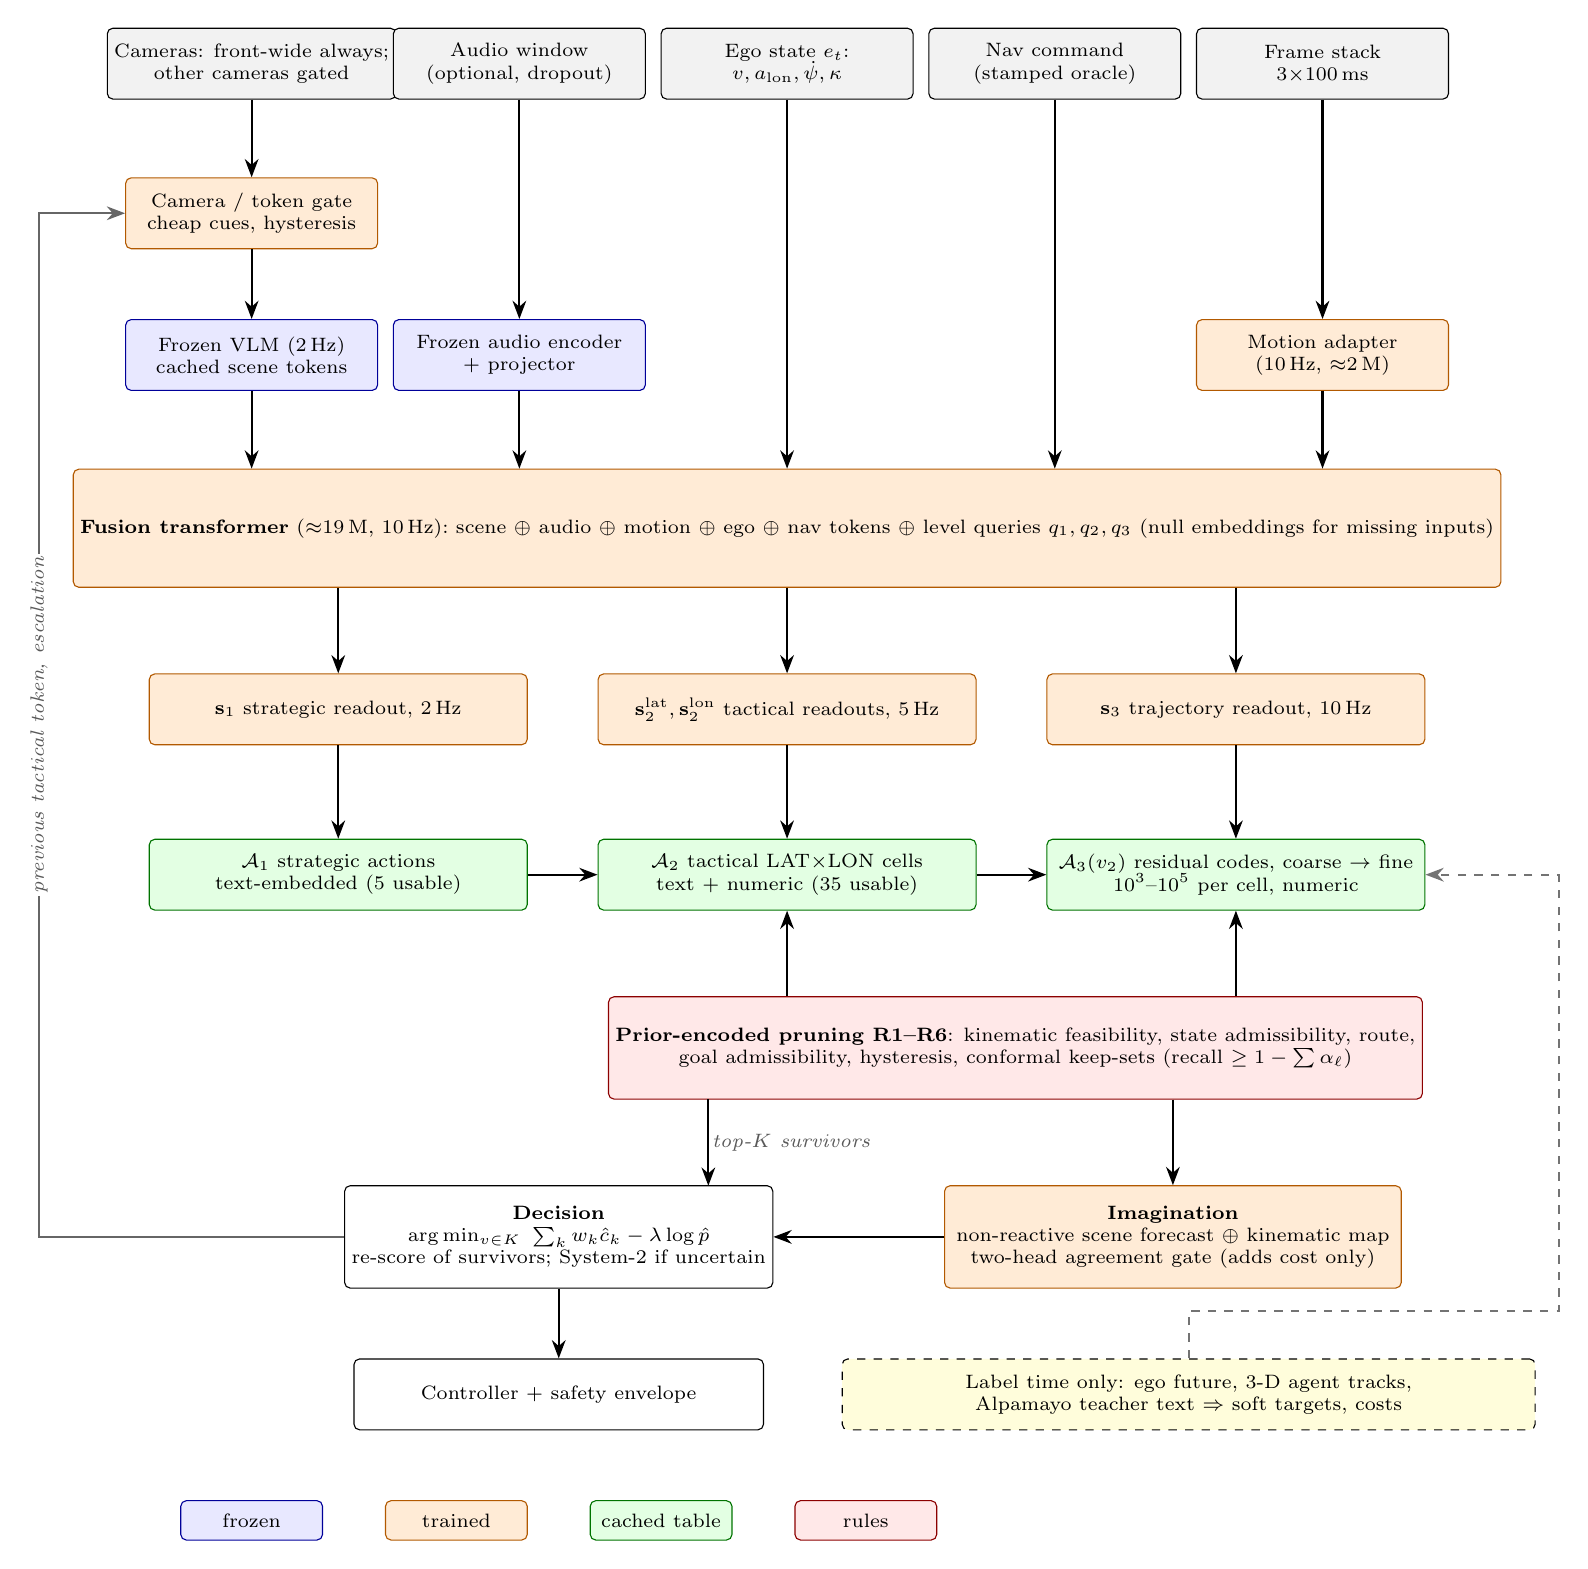
\begin{tikzpicture}[
  font=\scriptsize, >=Stealth,
  nd/.style={draw, rounded corners=2pt, align=center, inner sep=2.5pt, minimum height=9mm, minimum width=#1},
  nd/.default=32mm,
  inp/.style={nd, fill=gray!10},
  frz/.style={nd, fill=blue!9, draw=blue!60!black},
  trn/.style={nd, fill=orange!16, draw=orange!70!black},
  cch/.style={nd, fill=green!11, draw=green!45!black},
  msk/.style={nd, fill=red!9, draw=red!55!black},
  tch/.style={nd, fill=yellow!14, dashed},
  arr/.style={->, thick},
  darr/.style={->, thick, dashed, black!55},
  lab/.style={font=\scriptsize\itshape, text=black!65, fill=white, inner sep=1pt}
]
% ---------------- row A: inputs
\node[inp] (cam) at (1.7,0)  {Cameras: front-wide always;\\other cameras gated};
\node[inp] (aud) at (5.1,0)  {Audio window\\(optional, dropout)};
\node[inp] (ego) at (8.5,0)  {Ego state $e_t$:\\$v,a_{\mathrm{lon}},\dot\psi,\kappa$};
\node[inp] (nav) at (11.9,0) {Nav command\\(stamped oracle)};
\node[inp] (stk) at (15.3,0) {Frame stack\\3$\times$100\,ms};
% ---------------- rows B: gate, encoders
\node[trn] (gate) at (1.7,-1.9) {Camera / token gate\\cheap cues, hysteresis};
\node[frz] (vlm)  at (1.7,-3.7) {Frozen VLM (2\,Hz)\\cached scene tokens};
\node[frz] (aenc) at (5.1,-3.7) {Frozen audio encoder\\+ projector};
\node[trn] (mot)  at (15.3,-3.7) {Motion adapter\\(10\,Hz, $\approx$2\,M)};
% ---------------- row C: fusion
\node[trn, minimum width=178mm, minimum height=15mm] (fus) at (8.5,-5.9) {\textbf{Fusion transformer} ($\approx$19\,M, 10\,Hz):\ scene $\oplus$ audio $\oplus$ motion $\oplus$ ego $\oplus$ nav tokens $\oplus$ level queries $q_1,q_2,q_3$ (null embeddings for missing inputs)};
% ---------------- row D: readouts
\node[trn, minimum width=48mm] (s1) at (2.8,-8.2)  {$\mathbf s_1$ strategic readout, 2\,Hz};
\node[trn, minimum width=48mm] (s2) at (8.5,-8.2)  {$\mathbf s_2^{\mathrm{lat}},\mathbf s_2^{\mathrm{lon}}$ tactical readouts, 5\,Hz};
\node[trn, minimum width=48mm] (s3) at (14.2,-8.2) {$\mathbf s_3$ trajectory readout, 10\,Hz};
% ---------------- row E: action tree (cached embeddings)
\node[cch, minimum width=48mm] (a1) at (2.8,-10.3)  {$\mathcal A_1$ strategic actions\\text-embedded (5 usable)};
\node[cch, minimum width=48mm] (a2) at (8.5,-10.3)  {$\mathcal A_2$ tactical LAT$\times$LON cells\\text + numeric (35 usable)};
\node[cch, minimum width=48mm] (a3) at (14.2,-10.3) {$\mathcal A_3(v_2)$ residual codes, coarse $\to$ fine\\$10^{3}$--$10^{5}$ per cell, numeric};
% ---------------- row F: pruning
\node[msk, minimum width=100mm, minimum height=13mm] (pr) at (11.4,-12.5) {\textbf{Prior-encoded pruning R1--R6}: kinematic feasibility, state admissibility, route,\\goal admissibility, hysteresis, conformal keep-sets (recall $\ge1-\sum\alpha_\ell$)};
% ---------------- row G: decision and imagination
\node[nd=52mm, minimum height=13mm] (dec) at (5.6,-14.9) {\textbf{Decision}\\$\arg\min_{v\in K}\ \sum_k w_k\hat c_k-\lambda\log\hat p$\\re-score of survivors; System-2 if uncertain};
\node[trn, minimum width=58mm, minimum height=13mm] (img) at (13.4,-14.9) {\textbf{Imagination}\\non-reactive scene forecast $\oplus$ kinematic map\\two-head agreement gate (adds cost only)};
% ---------------- row H: controller
\node[nd=52mm] (ctl) at (5.6,-16.9) {Controller + safety envelope};
% ---------------- label-time box
\node[tch, minimum width=88mm] (tc) at (13.6,-16.9) {Label time only: ego future, 3-D agent tracks,\\Alpamayo teacher text $\Rightarrow$ soft targets, costs};
% ---------------- legend
\node[frz, minimum width=18mm, minimum height=5mm] at (1.7,-18.5) {frozen};
\node[trn, minimum width=18mm, minimum height=5mm] at (4.3,-18.5) {trained};
\node[cch, minimum width=18mm, minimum height=5mm] at (6.9,-18.5) {cached table};
\node[msk, minimum width=18mm, minimum height=5mm] at (9.5,-18.5) {rules};
% ---------------- edges
\draw[arr] (cam) -- (gate);
\draw[arr] (gate) -- (vlm);
\draw[arr] (aud) -- (aenc);
\draw[arr] (stk) -- (mot);
\draw[arr] (vlm.south) -- (vlm.south |- fus.north);
\draw[arr] (aenc.south) -- (aenc.south |- fus.north);
\draw[arr] (mot.south) -- (mot.south |- fus.north);
\draw[arr] (ego.south) -- (ego.south |- fus.north);
\draw[arr] (nav.south) -- (nav.south |- fus.north);
\draw[arr] (s1.north |- fus.south) -- (s1.north);
\draw[arr] (s2.north |- fus.south) -- (s2.north);
\draw[arr] (s3.north |- fus.south) -- (s3.north);
\draw[arr] (s1) -- (a1);
\draw[arr] (s2) -- (a2);
\draw[arr] (s3) -- (a3);
\draw[arr] (a1) -- (a2);
\draw[arr] (a2) -- (a3);
\draw[arr] (a2.south |- pr.north) -- (a2.south);
\draw[arr] (a3.south |- pr.north) -- (a3.south);
\draw[arr] (7.5,-13.15) -- node[lab, right] {top-$K$ survivors} (7.5,-14.25);
\draw[arr] (pr.south -| img.north) -- (img.north);
\draw[arr] (img.west) -- (dec.east);
\draw[arr] (dec) -- (ctl);
\draw[arr, black!60] (dec.west) -- (-1.0,-14.9) -- (-1.0,-1.9) -- (gate.west);
\node[lab, rotate=90] at (-1.0,-8.4) {previous tactical token, escalation};
\draw[darr] (tc.north) -- ++(0,0.6) -| (18.3,-10.3) -- (a3.east);
\end{tikzpicture}
}
\caption{HiCAP. Blue: frozen. Orange: trained. Green: cached embedding tables of the action tree. Pink: pruning and admissibility rules. The VLM refreshes at 2\,Hz, the motion adapter and fusion at
10\,Hz, and the level readouts update at 2/5/10\,Hz. A parent's choice restricts its children (a hard beam) but is not an input to the child's readout. Survivors of the pruning cascade are returned to the fusion transformer as candidate tokens for re-scoring;
a System-2 verifier runs only when the top-two margin is small or the two imagination heads disagree. The dashed box is label-time supervision, never available at inference.}
\label{fig:arch}
\end{figure}

\subsection{Backbone, motion adapter and fusion}\label{sec:backbone}
\paragraph{Frozen semantic backbone.}
The backbone $\mathcal V$ is a frozen vision--language model. At the slow rate it reads the selected cameras and a fixed short prompt once (prefill only) and we cache two
things: the hidden states of the visual tokens at a chosen late layer, pooled to at most $N_v=128$ tokens by fixed adaptive pooling, and the last-token hidden state
(the CLM readout). The backbone choice is a design decision with pending inputs, treated in \S\ref{sec:backbone-choice}; the interface is fixed regardless of the choice
(visual tokens of width $d_v$, a text tower, optionally an audio input).

\paragraph{Motion adapter.}
Frozen image and video encoders were measured to fail at metric ego-motion in this programme (a frozen single-frame encoder scored $2.1675$\,m ADE, REF-A\evI), and even a trained
driving trunk collapses without the ego channel ($1.1310$\,m against $0.2975$\,m when the ego state is zeroed on refcv4b\evI). The adapter $M_\phi$ ($\approx 2$\,M parameters)
therefore takes the three-frame stack (100\,ms apart) at $64\times160$, with inter-frame differences, and returns $N_m=16$ motion tokens. It is the only vision component
that is trained, and it is trained on frame pairs, not on single frames.

\paragraph{Fusion transformer.}
$F_\theta$ ($d=512$, six layers, eight heads, $\approx19$\,M parameters\evE) reads: the $N_v$ projected VLM tokens (each with a Fourier embedding of its \emph{age}, since VLM tokens are reused
between refreshes), the $N_m$ motion tokens, one ego token (an MLP over $e_t$ with a learned null row for ego-dropout), one navigation token, optionally $N_a$ audio tokens, and
three learned level queries $q_1,q_2,q_3$. The state readouts are
\begin{equation}
\mathbf s_\ell=\operatorname{norm}\big(H_\ell(F_\theta(\cdot)[q_\ell])\big),\qquad H_\ell:\Real^{512}\!\to\!\Real^{1024}\!\to\!\Real^{512},
\end{equation}
with the tactical level split into a lateral and a longitudinal query ($\mathbf s_2^{\text{lat}},\mathbf s_2^{\text{lon}}$), because the programme measured that a single softmax mixing the two
destroys the longitudinal decision. Readouts are Matryoshka-nested: the sum of the losses is taken at prefix widths $m\in\{128,256,512\}$ so that early levels can be scored at lower width
(\S\ref{sec:elastic}). The trainable part of the model is $\approx27$\,M parameters\evE (fusion, adapter, three readout heads, three action towers).

\subsection{The action tree and its vocabularies}\label{sec:vocab}
The PI's instruction was to use the last tactical vocabulary of the programme's dataset as the action space. That vocabulary is the frozen v7 vocabulary (\texttt{vocab\_v7.py}, frozen 2026-08-23): $56$ declared slots
($8+7+22+8+8+3$), $52$ distinct strings, ids equal to tuple indices, extension only through a new versioned tuple\evI. Table~\ref{tab:vocab} maps it onto the tree; the full token lists with counts are in Appendix~\ref{app:vocab}.

\begin{table}[t]
\centering\small
\caption{The action tree. \emph{Declared/populated} counts are per-field over the $4{,}719$ clips of the v7 corpus\evI; a token with $n=0$ is masked in the loss and in retrieval
(head width stays full). Level~3 is a design vocabulary, not a shipped one: its size $K_3$ is a parameter studied in \S\ref{sec:eff}.}
\label{tab:vocab}
\begin{tabularx}{\textwidth}{@{}p{2.1cm}p{2.3cm}p{2.7cm}p{2.1cm}X@{}}
\toprule
level & declared / populated & source & band, rate & node embedding \\ \midrule
L1 strategic action $a_{\text{str}}$ & $7$ / $5$ & ego-future geometry (label) & $[8,30]$\,s, 2\,Hz & frozen text tower on the token definition $\oplus$ arguments (\texttt{within\_m}, \texttt{by\_time\_s}) $\to$ MLP \\
L2 tactical cell $(a_{\text{tac}}^{\text{lat}},a_{\text{tac}}^{\text{lon}})$ & $8\times8=64$ / $5\times7=35$ & ego-future geometry (label) & $[2,6]$\,s, 5\,Hz & two factored embeddings (lat, lon) from text $\oplus$ arguments (\texttt{v\_target\_ms}, \texttt{within\_m}); pair-admissibility bias $b(c_{\text{lat}},c_{\text{lon}})$ \\
(side) tactical goals $g_{\text{tac}}$ & $22$ / $22$ (eight with $n<30$) & geometry + Alpamayo text (aux label) & $[2,6]$\,s & multi-label head on $\mathbf s_2$; 22 exclusive pairs; goal point $(x,y,t_{\text{reach}})$ regressed \\
L3a coarse residual code & $K_c$ per cell & train residuals over the CTRA prior & $[0,6]$\,s, 10\,Hz & numeric MLP on the coarse centre \\
L3b fine residual code & $K_f$ per coarse code & same, within a coarse cluster & same & numeric MLP on the full residual profile \\
\bottomrule
\end{tabularx}
\end{table}

\paragraph{Why these three levels, and their limits.}
The operative band $[0,2]$\,s has no tokens by design in the programme's vocabulary; it is a continuous quantity, which is what Level~3 encodes. The strategic supply is thin:
four of eight strategic goals and two of seven strategic actions have zero examples (no map, no time expression in the source text), leaving five usable strategic actions with
\cell{HOLD\_MAIN\_ROAD} alone at $2{,}468$ of $4{,}719$ clips\evI; lane changes are unreachable as tactical lateral actions because the emitter has no branch for them. So Level~1 is a five-way decision today. We keep the level because it
is the programme's thesis and the tree admits growth without redesign, but every strategic claim in this paper is conditional on that supply, and the pre-registration reports the strategic family
with its $n$ and reason (\S\ref{sec:protocol}).

\paragraph{Node embeddings.}
For Levels 1 and 2 the embedding is $\mathbf a_v=\operatorname{norm}\big(G_\ell([\mathbf t_v;\varphi(\text{args}_v)])\big)$, where $\mathbf t_v$ is the last-token hidden state of the frozen language tower on the token's definition string (computed once and cached) and
$\varphi$ a Fourier feature map of the numeric arguments. Text embedding gives structured geometry for free (\cell{PREPARE\_TURN\_L} lands near \cell{TURN\_L}) and lets a new versioned token be added with a meaningful initialisation. The tactical cell is scored
\emph{factored},
\begin{equation}
f_2\big(s,(c_{\text{lat}},c_{\text{lon}})\big)=\tau_2\langle\mathbf s_2^{\text{lat}},\mathbf a_{c_{\text{lat}}}\rangle+\tau_2\langle\mathbf s_2^{\text{lon}},\mathbf a_{c_{\text{lon}}}\rangle+b(c_{\text{lat}},c_{\text{lon}}),
\end{equation}
with $b=-\infty$ for pairs the programme's goal-admissibility tables forbid and a learned scalar elsewhere, so the lateral and longitudinal decisions remain separately evaluable as the marginals of one distribution.

\paragraph{Trajectory codes: residual over a physical prior.}
Let $\pi_{\text{prior}}(e_t)$ be the CTRA roll-out of the ego state, and $r=y^\star-\pi_{\text{prior}}(e_t)$ the residual of the logged 6\,s path on the eight slots. For each populated cell $c$ we collect the
residuals of \emph{training-split} windows assigned to that cell, run farthest-point selection with a time-weighted $L_2$ distance to $K_c$ coarse centres, refine by $k$-means, and repeat inside each coarse cluster to get $K_f$ fine
centres; a leaf is therefore $(c,i,j)$ and the codebook holds $35K_cK_f$ distinct residual profiles. Cells with fewer than $n_{\min}$ training windows back off to the codebook of their lateral class. The residual parameterisation has two purposes: the prior
removes the speed-dependent part of the path, so a code means ``brake harder than the prior'' rather than ``end 14\,m ahead'', and the physical prior is exactly what makes the kinematic pruning rules of \S\ref{sec:prune} cheap. The shipped
label window covers only $\pm2$\,s around each clip's anchor; for other windows the cell is recomputed from the window's own future path with the same threshold rules the label emitter uses (label-side only), which is an integration item
because the emitter lives on a branch not yet in the repository (\S\ref{sec:limits}).

\subsection{Scoring and training}\label{sec:train}
\paragraph{Per-level distribution.}
With kept children $K_\ell(u)\subseteq C(u)$ (\S\ref{sec:prune}), level $\ell$ defines
\begin{equation}
\hat p_\ell(v\mid u,s)=\operatorname{softmax}_{v'\in K_\ell(u)}\Big(\tau_\ell\langle\mathbf s_\ell,\mathbf a_{v'}\rangle+\beta_\ell\log\hat q_\ell(v'\mid u)\Big)_v,
\end{equation}
with $\tau_\ell=e^{\theta_\ell}$ initialised at $1/0.07$ and clamped at $100$ as in CLM, and $\hat q_\ell(\cdot\mid u)$ the train-split child frequency with additive smoothing. By Corollary~\ref{cor:bias} the InfoNCE-trained critic carries
$-\log\bar p$, so $\beta_\ell$ is fitted on held-out training episodes (grid $\{0,0.25,0.5,1,2\}$); with the soft-target softmax loss below the prior is already absorbed and $\beta_\ell=0$ is the default.

\paragraph{Losses.} The total loss is
\begin{equation}
\mathcal L=\sum_{\ell=1}^{4}\lambda_\ell\mathcal L^{\text{voc}}_\ell+\lambda_{\text{c}}\mathcal L^{\text{cons}}+\lambda_{\text{g}}\mathcal L^{\text{goal}}+\lambda_{\text{k}}\mathcal L^{\text{cost}}+\lambda_{\text{r}}\mathcal L^{\text{ref}}+\lambda_{\text{i}}\mathcal L^{\text{img}}+\lambda_{\text{a}}\mathcal L^{\text{aud}},
\end{equation}
where $\mathcal L^{\text{img}}$ and $\mathcal L^{\text{aud}}$ are defined in \S\ref{sec:imag} and \S\ref{sec:elastic}.
\begin{itemize}
\item \textbf{Vocabulary loss.} $\mathcal L^{\text{voc}}_\ell=-\sum_{v\in C(u^\star)}y_\ell(v)\log\hat p_\ell(v\mid u^\star,s)$ with the logged parent $u^\star$. Levels 1--2 use the label, masked for empirically absent classes. Levels 3a/3b use soft targets
$y(v)\propto\exp\!\big(-d_{\text{tw}}(y^\star,\hat y_v)^2/2\sigma^2\big)$ over the children of the logged parent, with $\sigma=0.5$\,m, following VADv2's distance-weighted target \citep{chen2024vadv2}; any candidate within $0.25$\,m of the logged path is never a negative.
For Level~3 the parent is the sampled (not the logged) one with probability $\rho$, ramped from $0$ to $0.3$, to reduce cascade exposure bias; the soft target is then computed against the sampled parent's children.
\item \textbf{Contrastive stage-1 variant.} In stage~1 the Level-3 loss can be the bidirectional in-batch InfoNCE of CLM with the same false-negative mask; Corollary~\ref{cor:bias} says what it estimates and the $\beta$ fit repairs it. Which of the two is better is registered as an ablation, not assumed.
\item \textbf{Goal loss.} A multi-label head on $\mathbf s_2$ over the 22 tactical goals, binary cross-entropy with positive weight capped at $50$, negatives supervised only for goals emitted from geometry or entailed false by an exclusive pair, plus an exclusivity penalty; and a regression of the goal point at $2/4/6$\,s. Goals are \emph{predicted}, never supplied.
\item \textbf{Consistency.} Unconditional level heads $\tilde p_\ell(v\mid s)=\operatorname{softmax}_{v\in V_\ell}(\tau_\ell\langle\mathbf s_\ell,\mathbf a_v\rangle)$ serve the faster update rates; $\mathcal L^{\text{cons}}=\sum_\ell\mathrm{KL}\big(\operatorname{sg}[\hat p^{\text{cascade}}_\ell]\,\|\,\tilde p_\ell\big)$ ties them to the cascade marginal.
\item \textbf{Cost heads (Hydra-style).} Per leaf, heads $\hat c_k(s,v)=\mathrm{MLP}_k(\mathbf s_3\odot\mathbf a_v)$ predict privileged costs: minimum time-to-collision proxy and minimum clearance, computed from the logged \emph{agent tracks} replayed non-reactively against each leaf's path (\S\ref{sec:imag}), and progress deficit. Comfort (acceleration and jerk) is computed exactly from $\hat y$ and needs no head. Distilling per-family sub-scores rather than one scalar follows \citet{li2024hydramdp}.
\item \textbf{Refinement.} $\delta=g(\mathbf s_3,\mathbf a_v)$, $L_1$ to the residual left after the code. It turns the vocabulary into a set of \emph{open} candidates, so the vocabulary bounds the search, not the accuracy.
\end{itemize}

\paragraph{Curriculum.} Three stages on cached features, as in CLM. Stage~1 trains all levels with sampled sibling negatives and no hard negatives. Stage~2 adds mined near-miss negatives (siblings whose ADE against the logged path lies in $[0.25,1.0]$\,m, plus synthetic speed-scaled copies of the positive) with $40\%$ stage-1 replay; CLM reports that hard negatives from the start overfit
($62.4\%$ against $69.2\%$)\evP{} (release README, not re-run here). Stage~3 unfreezes fusion and heads jointly and adds cost, refinement, imagination and audio losses, again with replay. Optimisation follows the programme's pre-registration: AdamW, no weight decay,
$\text{lr}=2\!\times\!10^{-3}\sqrt{1024/\text{width}}\sqrt{\text{batch}/1024}$, one-cycle with $10\%$ warm-up, batch $2{,}048$, three seeds per arm; intervals pool over episodes, never seeds.

\paragraph{Decision rule.}
\begin{equation}
a^\star=\arg\min_{v\in K_3}\ \sum_{k}w_k\,\hat c_k(s,v)\;-\;\lambda\log\hat p(v\mid s),\qquad \hat p(v\mid s)=\prod_{\ell}\hat p_\ell(v_\ell\mid v_{\ell-1},s),
\end{equation}
with the cost weights $w_k$ fixed \emph{a priori} by the four-metric-family policy and $\lambda$ fitted on held-out training episodes, never on validation data. With $w=0$ this is the maximum-likelihood leaf.

\subsection{Prior-encoded pruning and candidate-conditioned re-scoring}\label{sec:prune}
The candidate space is reduced by a short, ordered chain of rules, each stated so that its failure mode is measurable. Rules R1--R3 are hard and cheap; R4--R5 are soft; R6 is a calibrated guarantee.
\begin{description}[leftmargin=2.2em,style=nextline]
\item[R1 Kinematic feasibility (hard).] Keep leaf paths whose implied longitudinal acceleration, braking and lateral acceleration, given $v_0$, lie inside physical limits $\mathcal B_{\text{phys}}=(6,10,9)$\,m/s$^2$. Measured on real windows in \S\ref{sec:prelim}: it removes $78\%$ of a speed-agnostic anchor set and keeps every logged future.
\item[R2 State-conditioned admissibility (hard, calibrated).] Bin the ego state; keep tactical cells whose training frequency in that bin exceeds $\epsilon_A$, then calibrate $\epsilon_A$ conformally (R6) so that the logged cell is retained with a stated probability.
\item[R3 Route consistency (hard in the nav-fed arm only).] With $n_t=$ left, exclude right-turn cells and conversely. The navigation command is oracle-perfect in the corpus, so a hard rule looks better here than it will deploy; the nav-zero arm is the deployment-honest row and the rule is off there.
\item[R4 Goal admissibility (soft).] The predicted goal set contributes a log-prior bonus to the cells that serve those goals, using the programme's goal-to-action admissibility tables; it is soft because a wrong predicted goal must not delete the right cell.
\item[R5 Hysteresis (soft).] Leaves within a ball around the time-shifted previous plan receive a prior bonus, and switching requires a margin, to suppress oscillation.
\item[R6 Conformal keep-sets (guarantee).] Per level, keep the smallest set whose score threshold has calibrated coverage $1-\alpha_\ell$ (Proposition~\ref{prop:conformal}), giving joint recall $\ge1-\sum_\ell\alpha_\ell$ under episode-level exchangeability.
\end{description}
\paragraph{Feeding the survivors back to the backbone.}
The pruned set $K$ (at most $32$ leaves) is not only scored by the dot product. Their embeddings and refined paths are appended to the fusion transformer's input as \emph{candidate tokens} and a two-layer late-interaction block, in which candidates attend to the scene tokens but not to each other, produces a re-score $\tilde f(s,v)$; late interaction over a small set is the standard remedy for the rank cap of a single dot product \citep{weller2025limits,khattab2020colbert}. Cost is two cross-attention layers over $\approx160+|K|$ tokens.
Optionally, a \emph{System-2 verifier} runs when the top-two margin of $\tilde f$ is below $m_{\min}$ or the imagination heads disagree: the top $K_2\le5$ survivors are rendered as short text (\emph{lat=LANE\_KEEP, lon=BRAKE\_TO, target 6\,m/s}), one extra prefill of the VLM reads the scene and each rendering, and the CLM match score between the prompt's last-token embedding and the candidate text embeddings is added to the re-score.
The verifier fires only in uncertain ticks and fits inside the slow loop; it is the only place where the language side of the backbone acts at inference.

% ---------------------------------------------------------------------------
\section{Imagination that can be trusted}\label{sec:imag}
% ---------------------------------------------------------------------------
Prediction structure and imagination are the natural way to give a selector a sense of consequence: rather than asking ``which candidate resembles what the expert did'', ask ``what happens if I do this''.
The obstacle is identification. A world model trained on expert logs sees each action only in the states where the expert chose it, so its answer for any other action is an extrapolation.
Our programme measured two consequences of trusting such extrapolations: a rollout can be perfectly self-consistent for a candidate that is implausible, and rollout confidence can rise while rollout fidelity falls\evI.
The imagination stream of this design (repository manifest in \S\ref{sec:prelim}) added a third, uncomfortable finding that shapes the whole section: in a controlled toy, \emph{most of what looks like the benefit of imagination is the shape of the training target}, which costs nothing at inference. HiCAP-I is therefore built in three tiers, cheapest and safest first.

\paragraph{Tier 0 (training only): outcome-aware soft targets.}
The expert's one-hot label is the worst target the programme has measured for a selector\evI. Tier 0 replaces it by a listwise target built from per-candidate outcomes, which labels may use freely (ego and other agents),
\begin{equation}
y(a)\;=\;0.7\,\frac{\exp(-J_{\text{teacher}}(a)/T)}{\sum_{a'}\exp(-J_{\text{teacher}}(a')/T)}\;+\;0.3\,\mathbb 1[a=a^\star],
\end{equation}
where $J_{\text{teacher}}$ is a cost computed from the logged future of other agents and the candidate's known kinematics, with one head per metric family (safety, comfort, progress, lateral). It has zero inference cost. In the toy of \S\ref{sec:prelim} it cut regret from $7.00$ to $3.43$ (paired difference $3.57$, 95\% interval $[2.99,4.19]$), more than any imagination arm added on top.

\paragraph{Tier 1 (every tick): imagine the exogenous part, integrate the ego part analytically.}
For a candidate $a$ the outcome is $(W,e_a)$: the future scene $W$ and the ego path $e_a=\kappa(a,e_t)$, a \emph{known} function of the entry and the ego state. Only $W$ needs to be learned, and under the non-reactive assumption of Proposition~\ref{prop:ident} it does not depend on $a$, so it is identified by logs alone. The exogenous part is represented by a handful of descriptors, not by embeddings or frames (a future frame contains the ego's own motion and would smuggle the action into the target):
an E-head $\mathbb R^{512}\!\to\!\mathbb R^{1024}\!\to\!\mathbb R^{24}$ reading the state only outputs the lead gap, closing speed and lead acceleration at $0.5,1,2,3$\,s, a posterior over three to five behaviour modes (for instance the lead brakes, holds, accelerates) and onset-time quantiles. The cost of a candidate is the \emph{expectation over the mode and the timing},
\begin{equation}
J_1(s,a)=\mathbb E_{m,\tau\sim\hat p(\cdot\mid s)}\big[\,c\big(e_a,\ x_{m,\tau}\big)\big],
\end{equation}
with $c$ an analytic time-to-collision and clearance cost evaluated on the unicycle integration of the candidate. Marginalising \emph{every} hidden factor matters: a sharp mode posterior with a mean timing was over-confident in the toy ($+0.7$ regret). Tier 1 needs logs only, no counterfactual data, and it is the one imagination arm that survives their absence (regret $1.80$ against $47$--$72$ for the unstructured arms). Its cost is $\approx3$\,MFLOP per tick on the pruned set.

\paragraph{Tier 2 (gated, top-8, only where counterfactual supervision exists).}
Two cost heads on $\phi(s,a)=\operatorname{norm}(\mathbf s+R\,\mathbf v(a))$ regress per-family \emph{counterfactual} costs of a candidate, obtained from a rule teacher or a simulator (Proposition~\ref{prop:future} shows why the score cannot be an outcome-InfoNCE: it is identified only up to a per-candidate constant and cannot rank candidates, and a candidate-normalised softmax needs counterfactual data). Outcome InfoNCE is kept only as auxiliary representation shaping, and its targets are the exogenous descriptors of Tier~1 in the current ego frame, \emph{never} embeddings of future frames (which contain the ego's own motion and would teach an echo); an action-shuffled control whose failure voids Tier~2 checks this.
Tier~2 runs only for candidate families with counterfactual supervision, only on the survivors, and only when a \emph{learned} benefit gate fires (target $\le30\%$ of ticks). The disagreement of its two heads is a \emph{veto} on out-of-vocabulary candidates, not a benefit trigger: it detected them with an AUROC of $0.88$ (recall $64\%$ at $5\%$ false positives), while need-times-trust and margin gates were no better than random as triggers, and a learned gate reached $65\%$ of the gain at $30\%$ of the budget.

\paragraph{Composition and losses.}
\begin{equation}
\text{score}(a)=\tau\langle\mathbf u(s),\mathbf v(a)\rangle+\log\text{priors}-\beta_1J_1(s,a)-\beta_2J_2(s,a),\qquad J_1,J_2\ge0,
\end{equation}
so each imagination term adds a non-negative cost to a candidate (which can still change the argmin, since a candidate the base score ranked lower may be penalised less), and each term carries a zero-weight ablation. The imagination losses are $\mathcal L^{\text{img}}=\mathcal L^{\text{exo}}+\mathcal L^{\text{out}}+\lambda_{\text{inv}}\mathcal L^{\text{inv}}+\mathcal L^{\text{cons}}$: a Huber loss on descriptors plus cross-entropy on the mode plus a quantile loss on onset; an auxiliary outcome InfoNCE against the exogenous descriptors at $k\in\{5,10,20,40\}$ ticks, with per-state negatives where counterfactuals exist; an inverse-dynamics term of weight at most $0.1$ that keeps the action recoverable from state and future; and a parent--child hinge that keeps child outcomes consistent with their parent (strategic outcomes cannot be labelled without a map, so no strategic outcome quality is claimed).
\emph{No gradient flows from any imagination head into the frozen backbone}, and imagination parameters are trained separately from the selector's, since a world model that scores its own planner's fan was measured to help by only $+0.21$\evI.

\paragraph{Guards, each a measured failure.}
(G1)~An analytic feasibility and comfort mask is applied \emph{after} every learned term: imagination alone picked an infeasible over-braking candidate in $89.8\%$ of toy ticks and the mask brought it to $0\%$. (G2)~A counterfactual-coverage audit: a family without counterfactual supervision is refused by Tier 2. (G3)~A shuffled-cue and shuffled-$v_0$ control, with $R^2$ reported on the \emph{exogenous residual} only, because predicting the lead's speed from the ego state alone looks like imagination (echo). (G4)~Disagreement is a veto, never a benefit gate. (G5)~A confidence-sign audit: adding an imagined-cost term flipped the correlation of confidence with regret from $-0.11$ to $+0.19$ in all three seeds, so the combined softmax is never exposed as confidence. (G6)~$\beta$ is selected on held-out \emph{training} episodes that carry counterfactual labels (never on validation data), or it silently returns zero. (G7)~Every hidden factor is marginalised. (G8)~Every term is reported per family with a paired episode-cluster interval and its $n$ (agent-track coverage is stated for training clips only), and a risk-sensitive floor and a model-free value estimate on the same rows are always shown, otherwise risk-sensitivity is credited to imagination. (G9)~The goal path stays information-disjoint from the situation classifier: the E-head reads the state only.

\paragraph{Cost, and the first experiment.}
The imagination overhead is $\approx38$\,MFLOP per tick amortised (Tier 2 dominates), about $0.005\%$ of the smallest prefill (\evE); calling a learned world model for every candidate, or iterating rollouts over the whole set, would be $3$--$10\%$ of prefill and is not admitted. Efficiency is not the constraint; identifiability is.
The decisive first experiment is a probe costing $\approx0.1$\,GPU-hours on cached embeddings (E-I0): ridge and two-layer probes from the state to the lead gap now, the closing speed, the gap at $+2$\,s and the time to brake on the validation windows, against a $v_0$-only baseline and a shuffled-cue control. If the frozen state does not carry metric gap and closing speed (the programme's earlier frozen encoders did not), Tier 1 is inert and only Tier 0 ships; the toy's whole gap between $3.00$ and $0.46$ regret is exactly this readout error.

\paragraph{What could go wrong, and how the protocol sees it.}
(i)~Tier 1 may be inert because the backbone features lack range (E-I0, H-HC8). (ii)~The programme's earlier attempt to train an agent detector jointly with the trunk failed a two-seed capacity gate at $17$\,M parameters and the deranged-join control reproduced the whole degradation\evI; here the heads sit on a frozen backbone and do not compete with a trunk, but that is a hypothesis. (iii)~The non-reactive assumption fails at exactly the interactions that matter (yielding, merging); the one-sided form limits the damage and the shuffled controls (NC7) measure it. (iv)~In the toy the factorised arm \emph{lost} to the risk-sensitive floor when the cue was clean (regret $3.00$ against $2.17$ at a signal-to-noise ratio of $3$) because of visible-state readout error, the same failure as an earlier programme stream.

% ---------------------------------------------------------------------------
\section{Elastic sensing and audio}\label{sec:elastic}
% ---------------------------------------------------------------------------
Not every camera, token or channel is worth its cost at every instant. Table~\ref{tab:thor} shows why it matters: the vision tower's cost is linear in the number of cameras, so seven cameras cost about seven times the
vision-tower time of one at every refresh. HiCAP therefore treats the sensing configuration as a decision. This section states the policy, the evidence for and against it, and what it needs from data that does not yet exist.
The research stream behind it (repository manifest in \S\ref{sec:prelim}) also produced negative results that changed the design, and they are reported as such.

\subsection{Camera and token policy}
\paragraph{Frames, not cameras, are the first lever.}
A driving VLA that feeds four cameras with four frames each reads $\approx2{,}600$ visual tokens per tick ($\approx19.5$\,TFLOP for a 1.7\,B language model, \evE). HiCAP feeds \emph{one frame per camera} to the backbone and gives temporal information to the motion adapter at low resolution (\S\ref{sec:backbone}); one to three cameras then cost $1.3$--$3.6$\,TFLOP.
\paragraph{Tiers.}
The front-wide camera is always on at $160$ tokens. A tier adds cameras at $64$ tokens each: T1 adds one camera (front-tele for high-speed following and distance keeping; the cross camera on the turn side for junction approach; a rear-side camera for lane-change intent and merges);
T2 adds two; T3, all seven, is a probe and degraded-gate state, not a steady state. With peripheral cameras at $64$ tokens, all seven fit a $100$\,ms tick on a 2\,B-class stack ($\approx40$\,ms) and marginally on a 4\,B-class one ($\approx68$\,ms), against $\approx120$\,ms for seven cameras at $160$ tokens (\evE, scaled from NVIDIA's published rows, $\pm25\%$).
The first extra camera's language-model tokens are nearly free because the language stage is weight-streaming-bound at these lengths; its vision-tower pass is not, so savings made \emph{before} the tower (resolution, update rate, on/off) matter more than pruning after it.
A scheduled \emph{slow lane} encodes the rear and cross cameras at $2$\,Hz with tower and pooler only (no language-model pass) into a small peripheral-risk head, at $\approx19\%$ of the front lane's compute (\evH, untested); it covers what a gate cannot see.

\paragraph{The gate and which cues it may use.}
A camera gate is a situation classifier in disguise, because it maps a situation to a camera set. The programme's rule that inference is vision-only for scenario classification therefore applies, and the gate is specified in three arms.
\textbf{G-V} (primary, the only arm admissible under the rule) reads the front-wide pooled embedding, which the decision computes anyway, and the gate's own previous camera set (keep-alive state). \textbf{G-E} adds ego kinematics; it is an ablation until the PI rules on it.
\textbf{G-T} adds the previous tick's tactical token; it is \emph{not} information-disjoint, because the tactical decision would choose which pixels the next tick's goal path sees, so attribution between goal and gate would be lost and errors could lock in. G-T is admissible only if it beats G-V/G-E by the pre-registered margin and passes a \emph{config-invariance} test (the goal head scored on fixed-camera states must not degrade relative to gated states) and a \emph{gate-shuffle} test.
Labels may use everything: the relevance of a camera is the nearest dynamic agent in its field of view within a distance or time-to-collision threshold, from the 3-D agent tracks, combined with egomotion-derived manoeuvre intent.

\paragraph{Training.}
Because every camera can be cached offline, the per-option error $E_j(x)$ of the frozen backbone plus heads is computable for every training frame, and the gate minimises $\sum_jp_j(x)\,[E_j(x)+\lambda\,\mathrm{cost}_j]$ (full-information, cost-sensitive learning), with a calibrated situation head as an auxiliary or ensemble member. Errors are weighted by situation criticality: a wrong camera is nearly free in cruise and costly at a junction.
The heads are trained with a camera-dropout curriculum (illustratively $40\%$ the situation's oracle camera, $20\%$ oracle plus one random extra, $15\%$ all, $25\%$ front plus a random zero to two) and are \emph{budget-conditioned}: a configuration embedding is appended to the pooled state and the full-camera embedding is a distillation target for reduced configurations,
\begin{equation}
\mathcal L^{\text{cfg}}=\sum_{c}w_c\sum_{d\in\{64,128,256\}}\mathrm{InfoNCE}\big(f_d(\mathbf e_c),\mathbf a_d\big)+\beta\big(1-\cos(\mathbf e_c,\operatorname{sg}\,\mathbf e_{\text{full}})\big).
\end{equation}
The backbone is frozen, so this nesting lives in the trainable pooler and heads.

\paragraph{Dynamics: asymmetric keep-alive, shadow-mode prefetch.}
The gate escalates in one tick and de-escalates only after three ticks with a margin of $0.10$; it never smooths symmetrically. A newly enabled camera has no temporal cache, so it is switched on in \emph{shadow mode} (encoded, not used) for two ticks before its first use, driven by intent such as the route side.

\paragraph{What is not done, and why.}
Confidence-triggered escalation to all cameras and hedging with the runner-up camera are \emph{not} part of the design, because they measured as useless in the toy below. Matryoshka embedding \emph{dimensions} are adopted as a free option and are expected to save nothing: scoring $10^5$ cached candidates at $256$ dimensions is $\approx2.6\times10^7$ multiply-adds, far below a millisecond next to a $17$--$120$\,ms encoder. The nesting that carries compute is over cameras and tokens.

\subsection{Evidence: a toy world, its cliff, and what it does not show}
A synthetic world with seven cameras, seven sticky situations and exactly one informative camera per situation (\evM{}, \texttt{rd\_camera\_gating\_toy.py}; three seeds, a cost-sensitive gate, closed-loop keep-alive and a cold-start penalty; every constant is a chosen assumption) gives orderings, not levels. Decision accuracy and cost in camera units:
\begin{table}[h]
\centering\small
\caption{Camera-gating toy (mean of three seeds; \evM). Only orderings are evidence; the world scores one binary decision and chooses its own constants.}
\label{tab:gate}
\begin{tabular}{@{}lrr@{}}
\toprule
policy & cost (camera units) & decision accuracy \\ \midrule
fixed front-wide only & 1 & 0.732 \\
fixed all seven & 7 & 0.936 \\
ceiling: all seven plus true situation given to the head (reference) & 7 & 0.976 \\
oracle gate, cold start & 1.65 & 0.967 \\
\textbf{learned gate (ego cues, keep-alive)} & \textbf{1.64} & \textbf{0.951} \\
vision-only gate & 1.78 & 0.812 \\
vision-only gate with its own previous choice fed back & 1.72 & 0.804 \\
\bottomrule
\end{tabular}
\end{table}
Six readings. (i)~A gate can serve $95\%$ of decisions at $1.64$ camera units instead of $7$, but its apparent lead over fixed-all ($+1.4$ to $+1.8$ points, paired, per seed) is a head-routing-difficulty artefact: fixed-all must learn to route from noisy cues. The honest references are the oracle gate ($-1.6$ points) and the ceiling ($-2.5$ points).
(ii)~There is a \emph{cliff}: accuracy is flat between $1.6$ and $2.0$ units, then falls to $0.915$ at $1.49$ and $0.825$ at $1.25$. (iii)~A wrong camera costs almost nothing in cruise, about $22$ points for the tele case and $42$--$46$ points (chance) whenever the needed cross or rear camera is off; gate errors are \emph{confident}, concentrated on the tele-versus-wide ambiguity.
(iv)~Cue admissibility decides the design: the vision-only gate reaches only $0.812$, and with its own previous choice fed back it \emph{locks in}, holding a wrong camera set for $\approx49$ ticks ($\approx5$\,s); it matches the ego-cue gate only if the always-on front embedding separates situations about three times better than in the base world, which is an empirical property of the frozen VLM on real frames and the first thing to measure. (v)~Symmetric smoothing halves flicker but costs $0.5$--$0.6$ points against no smoothing; asymmetric keep-alive gains $+1.4$ points for $+6\%$ cost; a cold start costs $0.55$--$0.8$ points and prefetching two ticks ahead recovers $0.45$. (vi)~Confidence escalation buys at most $+0.02$ points for $+28\%$ to $+160\%$ cost.
The toy cannot say anything about real cameras: one informative camera per situation, uniform camera cost, an ad-hoc cold-start model and a chosen situation-code strength (its conclusion about vision-only gates depends on it).

\paragraph{Extra cameras are a data project.}
Every cache the programme has is front-wide only. Downloading one more upstream camera for the training set is $321$\,GB (front-tele) to $497$\,GB (cross-right) of transient volume, and all six is $2.55$\,TB (\evE, scaled from measured chunk sizes; $\approx9$\,h of build on a pod). A side-study over $\sim30$ dense chunks costs $49$--$388$\,GB but is not the parity corpus.
So the \emph{first} experiment is not the gate but the value of an oracle camera by manoeuvre, before any cache is bought: if no stratum shows an oracle camera beating front-only beyond the harm margin, elasticity is retired and front-only is shipped, which is also the cheapest outcome (H-HC10).

\subsection{Audio in the shared embedding space}\label{sec:audio}
Sirens and horns are decisive cues that may be invisible until late, and the leading model families are becoming omni-modal. We add audio as tokens in the backbone's own space, under a stricter regime than vision because audio cannot yet be validated as driving skill.

\paragraph{Pattern: a gated residual, not audio inside the language model.}
A frozen audio tower (a BEATs-base-class encoder of $\approx90$\,M parameters, or an ASR-class encoder if the chosen VLM family ships none) reads a two-second window; a two-layer Perceiver pools it to $k=8$ tokens; and the level-query outputs are updated by one gated cross-attention read,
\begin{equation}
\mathbf q_\ell'=\mathbf q_\ell+\tanh(g_\ell)\,\mathrm{CrossAttn}\big(\mathbf q_\ell,\ \text{audio tokens}\big),\qquad g_\ell\equiv0\ \text{at initialisation},
\end{equation}
so that audio-null is \emph{bit-exactly} the original model. That is the parity property the programme needs (a modality can be added without disturbing any earlier result), and it gives a deterministic test. The audio state is refreshed at $0.5$\,s hops ($\ge2$\,Hz), enough for a siren audible at $70$--$100$\,m and an emergency vehicle closing at $40$--$60$\,m/s ($1.2$--$2.5$\,s of warning, \evE). Soft audio tokens inside the language model ($+25$ tokens, $\approx+6\%$ of a one-camera tick) are the ablation.
The compute is negligible: $\approx18$\,GFLOP per two-second window for a BEATs-class tower ($\approx0.7$\,ms on Thor, \evE) against $17$--$31$\,ms for the first camera.

\paragraph{Alignment to language and vision through the frozen text path.}
The gate parameters are trained so that the audio-conditioned embedding matches the frozen VLM's own embedding of the scene together with a \emph{caption of the sound event},
$\mathcal L^{\text{aud}}=1-\cos\big(\mathbf e',\ \mathbf e_{\text{teacher}}(\text{image},\ \text{``siren approaching from behind, about 40\,m''})\big)$,
with the caption produced from the event generator's metadata (class, bearing, distance bin, approaching), \emph{not} from any driving label. Audio is thereby tied to language without audio--text language-model training, and the echo of a label is avoided (below). Optional pre-alignment uses public audio-caption sets. Direction of arrival needs a multi-microphone front end (inter-channel phase and level) before the tower, since mono log-mel features discard it.

\paragraph{The label-consistency trap, and what can be tested.}
A real logged trajectory never yields to a \emph{synthetic} siren, so an audio-augmented clip has no valid driving label unless the expert was already yielding, and then audio is present only where the label is ``yield'': a label echo. Therefore the audio path is trained on \emph{event metadata} only, and its behavioural effect is tested in closed-loop simulation with an acoustic layer computed offline from the simulator's actor poses (the simulator strips audio; the layer is circular, so detection realism must first be validated on real recordings).
On the current corpus we can test four things: (T1)~parity, audio-null equals the original embedding bit-for-bit; (T2)~event heads for class, bearing and distance on public audio-visual data and injected synthetic events; (T3)~usage controls on injected events, which show that the path \emph{can} read audio when it is the only informative channel, not driving skill; (T4)~no regression, so that noisy or absent audio leaves the four families unchanged (paired).
The controls are audio-null, audio-shuffle matched on speed bin and noise floor, a \emph{bearing flip} (mirrored channels flip the predicted side), a level dose-response ($0/-10/-20/-30$\,dB, monotone decay), an \emph{onset shift} ($\pm1$--$2$\,s from the label-consistent time), a siren with no visible vehicle and a visible vehicle without siren, and an \emph{audio-only label probe} (an audio-only classifier of the driving label must be at chance on real clips, the vision-only-rule leak test in a new costume). Synthetic events are rendered from world state, taking an actual agent track as the emitter and applying delay, $1/r$ gain, a Doppler shift $f'=f\,c/(c-v_r)$, air absorption, interaural time and level differences over a virtual array, and a speed-dependent ego-noise floor.
Modality dropout at $p=0.3$ keeps vision-only operation intact.

\paragraph{Evidence and gates.}
Published siren detectors with roof-mounted microphones report high presence recall with median direction error near $10^\circ$ and median distance error near $9$\,m within $10$--$50$\,m, degrading beyond $\approx70$\,m (arXiv:2109.14797, \evP, one-hop). No driving corpus the programme uses carries audio (PhysicalAI-AV, nuScenes, Waymo, Argoverse~2, comma2k19; the simulator strips it); the one place not yet probed is the audio stream of the shipped video container, a ten-minute check that would overturn this section if it found one. The wake-up gate (a band-energy detector that switches the tower on) has its false-positive rate measured. The PI ruled on 2026-09-29 that audio may optionally be used at inference, which settles admissibility and leaves the design constraints that ``optional'' implies: the model must run bit-identically without audio (T1); every family's primary result is reported audio-off and audio-on is a paired arm, so that no headline number depends on a channel no corpus can supply; the programme's vision-only rule for the situation classifier is untouched, because HiCAP has no classifier head, and the goal-path controls (NC6) apply to the audio path as to any other input; and the audio-only label probe stays mandatory, since an audio channel that predicts the label is exactly the leak the rule exists to catch.

% ---------------------------------------------------------------------------
\section{Theory}\label{sec:theory}
% ---------------------------------------------------------------------------
This section states what the design guarantees and under which assumptions. Every proposition is
elementary; the point is to make the assumptions explicit, because several failures observed in
our own programme (action echo, split-mean bias, uncalibrated imagination) came from unstated ones.

\subsection{Setting}
Let $s\in\mathcal S$ be the multimodal state (frames, ego state, optional audio). A decision is a leaf of a
rooted tree $\mathcal T$ of depth $L$: $a=(v_1,\dots,v_L)$ with $v_\ell\in C(v_{\ell-1})$, where $C(v)$ is the
finite set of children of node $v$ and $v_0$ is the root. In HiCAP there are three semantic levels (strategic action, tactical cell, trajectory residual;
\S\ref{sec:vocab}), and the residual level is itself a two-stage coarse-to-fine code, so retrieval runs over $L=4$ stages. Each node $v$ has a unit-norm embedding $\mathbf a_v\in\mathbb S^{d-1}$
and each level $\ell$ a unit-norm state readout $\mathbf s_\ell(s)\in\mathbb S^{d-1}$. The critic is
$f_\ell(s,v)=\tau\langle\mathbf s_\ell(s),\mathbf a_v\rangle$ with temperature $\tau>0$.
The expert (logged) decision is drawn from $p(a\mid s)=\prod_{\ell}p(v_\ell\mid v_{\ell-1},s)$.

\subsection{What contrastive training estimates, and the prior correction}
\begin{proposition}[Per-node InfoNCE optimum]\label{prop:infonce}
Fix a parent $u$ and a state $s$. Draw a positive child $v^+\sim p(\cdot\mid s,u)$ and $K$ negatives
i.i.d.\ from a proposal $q_u$ on $C(u)$. Among all critics $f$, the InfoNCE loss
$-\mathbb E\log\frac{e^{f(s,v^+)}}{e^{f(s,v^+)}+\sum_{k=1}^{K}e^{f(s,v^-_k)}}$
is minimised by
\begin{equation}
f^\star(s,v)=\log\frac{p(v\mid s,u)}{q_u(v)}+c(s),\label{eq:pmi}
\end{equation}
for any function $c$ of $s$ alone.
\end{proposition}
\begin{proof}
For fixed $s$ the loss is the cross-entropy of a $(K{+}1)$-way classifier that must identify which of
$K{+}1$ candidates was drawn from $p(\cdot\mid s,u)$ rather than from $q_u$. Its Bayes posterior that candidate $j$ is the positive is
$\frac{p(v_j\mid s,u)/q_u(v_j)}{\sum_i p(v_i\mid s,u)/q_u(v_i)}$, and the softmax over $f$ reproduces this posterior
exactly when $f=\log(p/q)+c(s)$, since $c(s)$ cancels in the normalisation. Cross-entropy is minimised
by the Bayes posterior. This is the noise-contrastive argument of \citet{oord2018cpc} and \citet{poole2019variational}.\qedhere
\end{proof}
\begin{corollary}[Selection bias and its correction]\label{cor:bias}
If $q_u$ is the marginal $\bar p_u(v)=\mathbb E_s\,p(v\mid s,u)$ (in-batch negatives), then
$\arg\max_v f^\star(s,v)=\arg\max_v\log\frac{p(v\mid s,u)}{\bar p_u(v)}$, the pointwise-mutual-information
maximiser, which differs from the likelihood maximiser $\arg\max_v p(v\mid s,u)$ whenever $\bar p_u$ is not uniform. Adding
$\beta\log\hat q_u(v)$ with $\beta=1$ recovers $\log p(v\mid s,u)+c(s)$. Because $\hat q$ and the critic are
estimated, $\beta$ is fitted on held-out episodes rather than fixed.
\end{corollary}
\noindent\textit{Example.} Prior $(0.70,0.20,0.10)$ over \{cruise, follow-lead, lane-change\}, true conditional
$(0.60,0.30,0.10)$ in a given state: PMI is $(-0.15,+0.41,0)$, so the PMI argmax is ``follow-lead'' while the most
likely action is ``cruise''. Our corpus is dominated by straight cruising, so the effect is systematic
(\S\ref{sec:prelim} gives the measured size on a synthetic world).

\begin{proposition}[Tree factorisation]\label{prop:tree}
Let $\hat p(v\mid u,s)=\operatorname{softmax}_{v'\in C(u)}\big(f_\ell(s,v')+\beta_\ell\log\hat q_u(v')\big)_v$. Then
$\hat p(a\mid s)=\prod_{\ell=1}^{L}\hat p(v_\ell\mid v_{\ell-1},s)$ is a normalised distribution over the
leaves, and $\log\hat p(a\mid s)$ decomposes into per-level terms that can be trained and calibrated independently.
By the chain rule the marginal of a node is the product along its path and equals the sum of the leaf
probabilities beneath it. The unconditional level heads that serve the faster update rates are separate parameters,
so their agreement with this marginal is trained with a KL term (\S\ref{sec:train}) rather than assumed.
\end{proposition}
\begin{proof}
Each factor is a softmax on the children of one node, so it sums to one; the product over a root-to-leaf
path therefore sums to one over all leaves by induction on depth.\qedhere
\end{proof}

\subsection{Cost and memory of hierarchical retrieval}
\begin{proposition}[Retrieval cost]\label{prop:cost}
Let level $\ell$ have branching $B_\ell=\max_u|C(u)|$ and beam width $b_\ell$ ($b_0=1$). Flat scoring of
$N=\prod_\ell B_\ell$ leaves costs $Nd$ multiply-accumulates and streams $N\,d\,w$ bytes of embeddings ($w$ bytes per element)
per decision. Beam retrieval touches $M=\sum_{\ell}b_{\ell-1}B_\ell$ nodes, i.e.\ $Md$ multiply-accumulates and $Mdw$ bytes.
\end{proposition}
\noindent For the sizes in Table~\ref{tab:vocab} this is the difference between streaming several gigabytes per tick
and reading a few megabytes; on an edge device the binding constraint is memory bandwidth, not arithmetic
(\S\ref{sec:eff}).

\subsection{Recall under cascaded pruning}
Pruning is safe only if it rarely removes the right action. We give two mechanisms.
\begin{proposition}[Conformal cascade]\label{prop:conformal}
For level $\ell$ let $\rho_\ell(s,v)$ be any score and $\hat t_\ell$ the $\lceil(1-\alpha_\ell)(n+1)\rceil$-th smallest value of
$-\rho_\ell(s_i,v_i^\star)$ over $n$ calibration windows, each scored against the children of \emph{its own logged parent}. For a test window let
$K^\star_\ell(s)=\{v\in C(v^\star_{\ell-1}):\,-\rho_\ell(s,v)\le\hat t_\ell\}$ be the keep-set that would be used if the logged parent had been retained.
If calibration and test windows are exchangeable, then $\Pr\big(v_\ell^\star\in K^\star_\ell(s)\big)\ge 1-\alpha_\ell$ for each level. The cascade retains the logged leaf exactly when
$v^\star_\ell\in K^\star_\ell(s)$ at every level, hence
\begin{equation}
\Pr\big(\text{logged leaf retained}\big)\;\ge\;1-\sum_{\ell}\alpha_\ell .\label{eq:recall}
\end{equation}
\end{proposition}
\begin{proof}
Level-wise coverage is the split-conformal guarantee \citep{angelopoulos2021gentle}: the test nonconformity $-\rho_\ell(s,v^\star_\ell)$ is exchangeable with the calibration values, so it is at most their $\lceil(1-\alpha_\ell)(n+1)\rceil$-th smallest with probability at least $1-\alpha_\ell$.
If the logged ancestors were all retained, the cascade's candidate set at level $\ell$ is the set of children of the logged parent, thresholded at $\hat t_\ell$, i.e.\ $K^\star_\ell(s)$; so the logged leaf is retained iff no level misses.
The union bound over the $L$ events $\{v^\star_\ell\notin K^\star_\ell(s)\}$, each of probability at most $\alpha_\ell$, gives \eqref{eq:recall}.\qedhere
\end{proof}
\noindent We state the union bound only: a product $\prod_\ell(1-\alpha_\ell)$ would require coverage \emph{conditional on} the parent having been retained, which conditions on an event of the test window and is not covered by exchangeability.
\noindent Exchangeability holds only across episodes, never across the windows of one episode, so calibration
and evaluation use episode-disjoint splits and the guarantee is marginal, not conditional on the scene.

\begin{proposition}[Physics mask]\label{prop:mask}
Let $\mathcal B$ be a set of kinematic limits (longitudinal acceleration and braking, lateral acceleration) and
$\mathcal K_{\mathcal B}(s)=\{a:\ \text{the implied path satisfies }\mathcal B\text{ given the current speed}\}$. If the logged
path satisfies $\mathcal B$, the mask retains it with probability one, so the oracle-in-set error is unchanged.
\end{proposition}
\noindent This is a statement about the bounds, not about the network, so it is checked empirically rather than proved:
Section~\ref{sec:prelim} reports that physical limits keep $881/881$ logged 2\,s futures of the validation set
(one-sided 95\% lower bound $0.05^{1/881}=0.9966$ on the window-level retention rate) while removing
$78\%$ of a speed-agnostic anchor set. Tight comfort limits ($3/6/4$\,m/s$^2$ for acceleration, braking, lateral) are \emph{not} safe as hard masks
(they removed $2.4\%$ of logged futures) and are therefore used as costs. The bound treats windows as independent; the 40
validation episodes make the effective sample smaller, which is why the calibrated conformal mask below, not this bound, is the shipped guarantee.

\subsection{Predictive imagination that is identifiable}
A world model trained on expert logs cannot learn what happens under an action the expert never took,
because in the log the action is a function of the state. We therefore split the outcome into a part the ego cannot
change over the horizon and a part it controls.
\begin{proposition}[Identifiable outcome factorisation]\label{prop:ident}
Let $W_{t+1:t+H}$ be the future scene (other agents, signals) and $e_{t+1:t+H}$ the ego path. If the scene is
non-reactive over the horizon, $W_{t+1:t+H}\perp a\mid s$, then $p(W_{t+1:t+H}\mid s,a)=p(W_{t+1:t+H}\mid s)$ is identified by the
observational log, and $e_{t+1:t+H}=\kappa(a,s_{\text{ego}})$ is a known kinematic function. Any interaction cost
$c(W,e)$ can then be evaluated for every candidate $a$ without a learned counterfactual model.
\end{proposition}
\begin{proof}
Conditional independence gives the first equality; the right-hand side involves no intervention on $a$, so it is a
functional of the joint observational distribution. The ego path is a deterministic function of the candidate and the ego state.\qedhere
\end{proof}
\noindent The assumption fails for reactive agents (a driver yielding to the ego). We do not hide this: reactivity is
bounded by a learned correction term whose weight is limited and which is reported separately, and imagination is
never allowed to \emph{raise} confidence unless two independent heads agree (\S\ref{sec:imag}).

\begin{proposition}[Contrastive future critic]\label{prop:future}
Let $g(s,a,s')=\tau\langle\Phi(s,a),\mathbf z(s')\rangle$ be trained with InfoNCE against future embeddings $s'$ of
other windows as negatives. Its optimum is $g^\star=\log\frac{p(s'\mid s,a)}{p(s')}+c(s,a)$, so the score is a
pointwise-mutual-information estimate between the candidate and its outcome.
\end{proposition}
\begin{proof}
Identical to Proposition~\ref{prop:infonce} with the positive drawn from $p(s'\mid s,a)$ and negatives from the marginal $p(s')$.\qedhere
\end{proof}

\subsection{Distilling the selector into a small student}
\begin{proposition}[Decision preservation]\label{prop:distill}
Let student embeddings satisfy $\|\hat{\mathbf s}-\mathbf s\|_2\le\delta_s$ and $\|\hat{\mathbf a}-\mathbf a\|_2\le\delta_a$ (unit vectors).
Then $|\tau\langle\hat{\mathbf s},\hat{\mathbf a}\rangle-\tau\langle\mathbf s,\mathbf a\rangle|\le\tau(\delta_s+\delta_a)$, and the student's
arg\,max equals the teacher's whenever the teacher's top-1/top-2 score margin exceeds $2\tau(\delta_s+\delta_a)$.
\end{proposition}
\begin{proof}
$\langle\hat{\mathbf s},\hat{\mathbf a}\rangle-\langle\mathbf s,\mathbf a\rangle=\langle\hat{\mathbf s}-\mathbf s,\hat{\mathbf a}\rangle+\langle\mathbf s,\hat{\mathbf a}-\mathbf a\rangle$,
each term bounded by Cauchy--Schwarz. A rank change between two candidates requires their scores to move toward each other by
at least the margin, i.e.\ each by at least half of it.\qedhere
\end{proof}
\noindent Because the interface between backbone and heads is a fixed-dimension embedding space, the frozen
multi-billion-parameter backbone can be replaced by a sub-300\,M student trained to match the cached teacher embeddings and
candidate scores; Proposition~\ref{prop:distill} converts an embedding-error budget into a decision guarantee.

% ---------------------------------------------------------------------------
\section{Efficiency: what is cached, what runs when, and how large the backbone may be}\label{sec:eff}
% ---------------------------------------------------------------------------
Compute efficiency is a design constraint, not a tuning step. Four mechanisms carry it: multi-rate execution, caching at build time, hierarchical retrieval,
and pruning before expensive computation (elastic sensing, \S\ref{sec:elastic}, is the fifth). This section states each cost in closed form or from published
figures and separates that clearly from anything we have timed. \textbf{Nothing in this section is a HiCAP timing}: rows are arithmetic (\evE) or NVIDIA-published
figures for the backbone alone (\evP).

\subsection{Multi-rate execution}
The decision levels have different natural rates, and so does the cost. Table~\ref{tab:rates} is the schedule.
\begin{table}[h]
\centering\small
\caption{Multi-rate schedule. The frozen VLM is the only expensive component and runs at the slowest rate; the fast path is small enough that launch overhead, not arithmetic, dominates it.}
\label{tab:rates}
\begin{tabularx}{\textwidth}{@{}p{3.3cm}p{1.6cm}Xp{2.6cm}@{}}
\toprule
component & rate & recomputed & cost model \\ \midrule
frozen VLM (ViT + prefill), selected cameras & 2\,Hz & visual tokens at three depths, last-token state; between refreshes tokens are reused with an age embedding & Table~\ref{tab:thor} \\
motion adapter & 10\,Hz & 16 motion tokens from the 3-frame stack & $\approx2$\,M params \\
fusion transformer & 10\,Hz & level queries over $\approx160$ tokens & $\approx19$\,M params, $\approx8$\,GFLOP\evE \\
L1 readout / retrieval & every 2\,s & strategic scores, keep-set & 5 nodes \\
L2 readout / retrieval & every 0.5\,s & tactical cell scores, classes then members; survivors cached for five ticks and re-masked each tick & $\le35$ cells; $1{,}280$ factor rows \\
L3 compose, re-score, refine & every 0.1\,s & compose $\approx200$ entries, late-interaction shortlist, cross-attention re-rank of $K=16$, refinement & $\approx0.34$\,GMAC, Table~\ref{tab:cost} \\
System-2 verifier & only if uncertain & one extra prefill on $\le5$ renderings & one prefill row of Table~\ref{tab:thor} \\
\bottomrule
\end{tabularx}
\end{table}
The fusion cost of $\approx8$\,GFLOP is $2\times19\text{M}\times200$ tokens, ignoring attention; at the $\approx25$\,TFLOP/s eager-bf16 throughput class of the programme's encoder measurements\evI{} this is well under a millisecond
of arithmetic, so the fast path is expected to be launch-bound, and the only honest statement is that it must be measured (hypothesis H-HC11).

\subsection{Backbone cost on the target SoC}\label{sec:backbone-cost}
NVIDIA publishes measured Jetson Thor figures for Qwen3-VL-2B, -4B and -8B (TensorRT Edge-LLM 0.10.0, batch 1, vision tower FP16, language model NVFP4)\evP: for the 4\,B model a ViT pass of $11.6$\,ms and a $292$-token prefill of $22.3$\,ms, and a $2{,}048$-token prefill of $62.2$\,ms.
Interpolating linearly in token count and scaling the ViT with the number of camera images gives Table~\ref{tab:thor}; the research stream, using a reduced vision-tower cost and $160$ tokens per camera, estimates $\approx31$\,ms and $\approx61$\,ms for the recommended Qwen3.5-4B with one and three cameras ($\pm25\%$, \evE); the table's row for it uses the published rows directly and is the more conservative. The ViT row is measured on a $\sim$265-token image while our cylindrical crop yields $160$ tokens per camera, so the ViT column is an upper bound; the one-camera column ($n=224$) lies below the smallest published prefill length ($292$), so it is an extrapolation.
\begin{table}[h]
\centering\small
\caption{Estimated backbone latency per VLM refresh on Thor from the published rows (linear interpolation; ms). $n$ = total tokens (160 per camera + 64 prompt/query).}
\label{tab:thor}
\begin{tabular}{@{}lrrrrrr@{}}
\toprule
& \multicolumn{2}{c}{1 camera ($n{=}224$)} & \multicolumn{2}{c}{3 cameras ($n{=}544$)} & \multicolumn{2}{c}{7 cameras ($n{=}1184$)} \\
model & ViT & total & ViT & total & ViT & total \\ \midrule
Qwen3-VL-2B & 11.4 & 23.5 & 34.2 & 49.1 & 79.8 & 100.3 \\
Qwen3-VL-4B & 11.6 & 32.4 & 34.8 & 62.8 & 81.2 & 123.8 \\
Qwen3.5-4B (recommended R1) & 10.9 & 40.0 & 32.7 & 73.4 & 76.3 & 140.2 \\
Qwen3-VL-8B & 15.7 & 45.0 & 47.1 & 89.6 & 109.9 & 178.8 \\
\bottomrule
\end{tabular}
\end{table}
Two conclusions follow, both estimates. First, a single camera at a $2$--$10$\,Hz refresh is cheap (a 4\,B model at $\approx32$--$40$\,ms), so the case for a frozen VLM in the loop does not rest on the model being slow. Second, the cost is dominated by the vision tower and is linear in the number of cameras,
so seven cameras cost $\approx124$--$140$\,ms per refresh and cannot run at 10\,Hz; the value of choosing cameras per tick (\S\ref{sec:elastic}) is exactly this slope. An open question is the precision drift between NVFP4 features on the vehicle and the BF16 features a head was trained on; it is registered as a measurement (H-HC11).

The same arithmetic explains why a decode-based VLA behaves differently: Cosmos3-Edge's 4.8\,GB of BF16 weights over $273$\,GB/s give a $57$\,tok/s ceiling and NVIDIA measures $37$--$43$\,tok/s\evP; a trajectory of a few hundred tokens costs seconds, while prefill plus a table lookup costs tens of milliseconds.

\subsection{Latency, not parameter count, sets the backbone size}\label{sec:latency}
The PI ruled on 2026-09-29 that the programme's sub-300\,M cap does not bind this arm if the inference time of the whole system is very low. That turns a size rule into a latency rule, and two clocks have to be told apart because they respond to backbone size in opposite ways.
\emph{Command latency} $L_{\text{cmd}}$ is the time from the newest camera frame to the emitted command. It runs through the motion adapter, the fusion transformer, retrieval and the heads; the backbone enters only through the cache, so to first order $L_{\text{cmd}}$ does not depend on the backbone's size. \emph{Token age} $A$ is the age of the cached VLM tokens when the fast path reads them; with refresh rate $f_r$, refresh compute time $T_r$ and an overhead $o$ for pooling, hand-off and pre-processing, the worst case is $A=T_r+o+1/f_r$. A larger backbone raises $T_r$, hence $A$ and the refresh duty $D=f_r(T_r+o)$. We register three criteria in advance: $D\le0.5$ (the remainder is for the fast path and the vehicle's other tenants; an assumption), the fast-path p95 $\le25$\,ms \emph{measured while a refresh is running}, and $L_{\text{cmd}}$ p95 $\le100$\,ms, the tick. The synchronous reading, in which the refresh sits inside the tick, is the special case $f_r=10$\,Hz. The size ruling is therefore met by construction only if two things hold that no arithmetic here can show: that the refresh does not inflate the fast path through contention for the SoC's 20 streaming multiprocessors\evI{} and its $273$\,GB/s\evP{} (no preemption is assumed), and that stale tokens do not cost decision quality (H-HC11, H-HC15).

Table~\ref{tab:maxbody} gives, for the dense Qwen3-VL lineage that carries the published rows, the largest body that meets $D\le0.5$ under the pessimistic effective throughput. Inside the measured body range ($1.4$--$7$\,B) the time is interpolated between the three published rows; above it, the eight-billion row's effective rate is assumed to be a lower bound on throughput (monotone in size across the three published points, $65/95/126$\,TFLOP/s at $n=292$ and $206/239/272$ at $n=2{,}048$; not true across families, since the Qwen3.5 hybrid is about $1.5\times$ slower per token). Entries beyond twice the largest measured body ($13.9$\,B) are stated only as ``at least'', with no fitted exponent and no point estimate.
\begin{table}[h]
\centering\small
\caption{Largest dense backbone body (billions of parameters) meeting refresh duty $D=f_r(T_r+15\,\text{ms})\le0.5$ at the pessimistic throughput (\evE, \texttt{hicap\_latency\_budget.py}; anchored on \evP{} Thor rows, ViT and LLM as in Table~\ref{tab:thor}). ``$>13.9$'': the bound lies beyond twice the largest measured body. ``none'': the vision tower alone exceeds the budget. Frames per camera is the number of images the VLM reads per refresh; the motion adapter supplies temporal information, so one frame per camera is the primary setting.}
\label{tab:maxbody}
\begin{tabular}{@{}lrrrr@{}}
\toprule
refresh $f_r$ & 1 camera, 1 frame & 3 cameras, 1 frame & 7 cameras, 1 frame & 3 cameras, 3 frames \\ \midrule
2\,Hz (asynchronous) & $>13.9$ & $>13.9$ & 12.6 & 7.9 \\
5\,Hz & $>13.9$ & 5.9 & none & none \\
10\,Hz (synchronous) & 4.0 & none & none & none \\
\bottomrule
\end{tabular}
\end{table}
The reading is direct. At $2$\,Hz an 8\,B-class backbone (the estimate from the published Qwen3-VL-8B rows: $223.4$\,ms for three cameras with three frames each, duty $0.48$ with the assumed $15$\,ms overhead) is admitted, and with one frame per camera a body of up to about $30$\,B meets the duty rule at three cameras as a bracket outside the measured range; at $10$\,Hz only a $4$\,B-class model with one camera does, so a 10\,Hz VLM refresh forces a small backbone and the ruling buys nothing there. The price of the large backbone is age: an 8\,B model at three cameras (one frame) has $A\le90+15+500\approx0.6$\,s, which at $15$\,m/s is $9$\,m of travel; the fusion transformer's age embedding and the motion adapter carry the fresh part of the state, but metric quantities such as the lead gap that the imagination tiers read from the cached state are the ones a stale token cannot provide (\S\ref{sec:imag}); the forecast horizon is therefore counted from token capture, an assumption tested by H-HC15.

\begin{table}[h]
\centering\footnotesize
\caption{Backbones without a published Thor row, as brackets (optimistic--pessimistic ms per refresh, ViT $+$ prefill, no overhead; \evE). Optimistic $=\max(2P_{\text{body}}n/272\,\text{TFLOP/s},\ \text{weight floor})$; pessimistic scales the 8\,B row by $P_{\text{body}}/6.95$; the MoE row is bounded above by the published $137.7$\,ms $2{,}048$-token row of the text model. The weight floor streams every weight once at $0.7\times273$\,GB/s. Memory is weights only at 4.5 bit (NVFP4), 8 bit and 16 bit; cache is the int8 token cache of \S\ref{sec:eff} at three depths and $128$ tokens for $188{,}640$ refreshes, at the assumed hidden width ($2{,}048$, $5{,}120$ and $2{,}048$ for the three rows); the 32\,B row assumes the Qwen3-VL-32B architecture and a SO400M vision tower (UNVERIFIED).}
\label{tab:bracket}
\begin{tabular}{@{}p{3.3cm}rrrrrp{2.3cm}r@{}}
\toprule
backbone & 1 cam & 3 cam & 7 cam & 3 cam, 3 fr & floor & weights GB (4.5/8/16 bit) & cache GB \\ \midrule
Cosmos3-Edge reasoner, 2.4\,B & 28 & 62 & 130 & 165 & 7 & 1.4 / 2.4 / 4.8 & 148 \\
Cosmos-Reason2-32B & 113--147 & 172--238 & 382--419 & 486--510 & 97 & 18.6 / 33 / 66 & 371 \\
Qwen3-Omni-30B-A3B, 3.3\,B active & 106--153 & 137--185 & 200--248 & 231--279 & 90 & 17.2 / 30.5 / 61 & 148 \\
\bottomrule
\end{tabular}
\end{table}
Eight-billion-class models need no bracket: Cosmos-Reason2-8B, the Cosmos~3 Nano reasoner and the Alpamayo~1.5 language model are described as sharing the Qwen3-VL-8B architecture (a model-card statement, inherited, not re-verified), so the published 8\,B row applies to all three if that equivalence holds, and its cache is $297$\,GB at a hidden width of $4{,}096$ (an assumed width). The $32$\,B rows sit at the edge of the $250$\,ms budget at three cameras with one frame ($172$--$238$\,ms plus the $15$\,ms overhead) and exceed it for any further frame or camera, so they are teachers unless the camera set is small; the MoE row is bound by weight streaming, not by its $3.3$\,B active parameters, which is the reason a sparse model is not cheap on a bandwidth-limited SoC. Four caveats bound everything in this subsection: the ViT cost per image is the published one (a conservative upper bound at our $640$-patch crop); all rows exclude engine hand-off and any contention; NVFP4 feature drift against BF16 is unmeasured; and no TensorRT build exists in our hands for any model except through NVIDIA's published rows. The on-device benchmark (\texttt{hicap\_backbone\_latency\_bench.py}, H-HC11) is written, unit-tested with a mock backend, and has not been run.

\paragraph{The scale ladder and the cost of adapting the backbone.}
Removing the cap changes the experimental design in two ways. First, backbone size becomes a variable: the same heads on Qwen3-VL-2B, 4B and 8B (Cosmos-Reason2 provides 2\,B and 8\,B members of the same architecture, inherited) give a size ladder inside one family, read by matched-step ratios and never by an exponent (H-HC16). Second, the argument for freezing weakens where geometry matters: a frozen-VLM BEV head lost $6.34$\,mAP against its control and unfreezing recovered $10.46$\evP{} (one-hop, vendor-reported). Adapting the backbone (low-rank adapters on the language model and the vision tower) forfeits the cache, which is what makes CLM cheap to iterate on. The arithmetic for one epoch of $188{,}640$ refreshes at $544$ tokens for an 8\,B body is $4P_{\text{body}}n\approx1.5\times10^{13}$\,FLOP per sample for a forward pass plus activation gradients (weight gradients only for the adapters), or $2.8\times10^{18}$\,FLOP per epoch, which is $8$--$13$ GPU-hours at an assumed $60$--$100$\,TFLOP/s effective bf16 on an A40-class part (\evE; activation memory not costed; the full-backward figure is $\approx1.5\times$ that). This is affordable once and not for a grid, so the adapted arm is pre-registered after the frozen ladder (H-HC17), never before H-HC0.

\subsection{Retrieval cost of a very large vocabulary}
The trajectory vocabulary is a product of $K_P$ paths and $K_V$ speed profiles, so scoring the two factors separately, keeping $(k_P,k_V)$ and composing costs $K_P+K_V+k_Pk_V$ rows instead of $K_PK_V$ (Proposition~\ref{prop:cost}). Table~\ref{tab:cost} compares this with scoring every composed entry, at $d=512$ against the $273$\,GB/s of Thor\evP; the last column is the time to stream the flat table once at the published peak bandwidth.
\begin{table}[h]
\centering\small
\caption{Flat versus factored retrieval per decision (\evE, from Proposition~\ref{prop:cost}); bf16, $d=512$. Flat time is the table read at the published peak bandwidth of 273\,GB/s, a single reader; the backbone competes for the same bandwidth.}
\label{tab:cost}
\begin{tabular}{@{}rrrrrrr@{}}
\toprule
$K_P\times K_V$ & composed $N$ & kept $(k_P,k_V)$ & rows touched & ratio & flat MB (time) & factored MB \\ \midrule
$1{,}024\times256$ & $2.6\times10^{5}$ & $(20,10)$ & 1{,}480 & $177\times$ & 268 (0.98\,ms) & 1.5 \\
$2{,}048\times512$ & $1.05\times10^{6}$ & $(32,16)$ & 3{,}072 & $341\times$ & 1{,}074 (3.9\,ms) & 3.1 \\
$4{,}096\times1{,}024$ & $4.2\times10^{6}$ & $(40,20)$ & 5{,}920 & $709\times$ & 4{,}295 (15.7\,ms) & 6.1 \\
\bottomrule
\end{tabular}
\end{table}
The honest reading is a scale argument. At the vocabulary sizes of published scorers ($4{,}096$--$8{,}192$ entries) and even at $262{,}144$, flat scoring streams a few hundred megabytes in about a millisecond, so the hierarchy buys no speed at inference; the bandwidth argument begins beyond a few million entries, where an approximate index would otherwise be needed (none is a published 10\,Hz edge precedent). The hierarchy earns its place elsewhere: it gives the backbone a \emph{small} set to reason over (the cascade of \S\ref{sec:prune} costs $\approx0.34$\,GMAC per tick at $K=16$, and the cross-attention re-ranker at $K=8/16/32$ is $0.20/0.29/0.48$\,GMAC, \evE), it gives level-wise priors and a native tactical readout, and it estimates priors for entries with almost no data (about $1.5$ training windows per leaf at this size). A failure of the tree is therefore not fatal: flat scoring is the reference arm and the fallback. Training is affected earlier than inference: a flat softmax over $262{,}144$ entries at batch $2{,}048$ materialises $\approx0.5$\,G logits per step, whereas the level softmaxes are over a few thousand nodes.
Whether a larger vocabulary \emph{helps} accuracy is a separate, empirical question (H-HC5): an oracle-in-set curve is necessary but not sufficient, since the programme's own measurements show the selection gap growing with the candidate set for a fixed scorer (REF-C-XL restricted to $64/128/256$ anchors: oracle-in-fan $0.4368/0.2624/0.1640$\,m while the share of windows in which the pick is at least twice as bad as the best rises $0.1771/0.3190/0.4540$; registry \S4)\evI.

\subsection{Caching at build time}
Training the heads on cached features is what makes CLM cheap to iterate on. For HiCAP the dominant cache is the VLM tokens: at a $2$\,Hz refresh, $26.2$\,h of video is $188{,}640$ VLM ticks; $128$ tokens of width $2{,}048$ (an assumed width; the recommended backbone's hidden size is unverified) at three depths and one byte per element is $148$\,GB, and $64$ tokens is $74$\,GB (\evE, \texttt{hicap\_cost\_model.py}). A $10$\,Hz refresh would be $742$\,GB at int8 and is therefore not cached. Action embeddings are cached per step as a table and are tiny by comparison.
Ablations over heads, losses and vocabularies then cost GPU-minutes on cached tensors rather than the $\approx45$\,GPU-hours per arm that the programme's reference planner needs by arithmetic on an inherited receipt ($40{,}284$ steps at $4.0$\,s/step on an A40; \evE, \evI); the cache is built once per backbone and once per camera set.

\subsection{Backbone choice}\label{sec:backbone-choice}
The instruction was to start from a VLM with general world knowledge and, ideally, driving knowledge, ``such as Cosmos Drive Nano or something similar''. No model of that name exists in NVIDIA's model tables or repositories (absence probed in the Cosmos model table, the Alpamayo recipes, the TensorRT Edge-LLM support list and four searches; absence at four locations is not proof).
The closest real objects are the 10\,B Alpamayo~1/1.5 ``Nano'' VLA (a Cosmos-Reason backbone with a driving action expert, too large per tick), Cosmos~3 Nano (16\,B) and Cosmos3-Edge (4\,B, whose 2.4\,B reasoner is a Nemotron-dense language model with a SigLIP\,2 vision tower and no audio tower), and Cosmos-Drive-Dreams, which is a video generator and not an encoder.
Our reading is that the request means a Cosmos-lineage reasoner with driving knowledge that fits the Thor; no one has published that combination, and NVIDIA's own edge answer is reported to be distillation of a large teacher into a $0.5$--$2$\,B student\evP{} (one-hop).
\begin{table}[h]
\centering\small
\caption{Backbone shortlist, in test order. Thor rows are NVIDIA-published where present\evP; ``paired'' means the two arms differ in driving tuning only.}
\label{tab:backbones}
\begin{tabularx}{\textwidth}{@{}p{0.6cm}p{3.6cm}p{2.2cm}p{2.4cm}X@{}}
\toprule
rank & backbone & role & audio & why \\ \midrule
R1 & general Qwen3.5-4B (Apache-2.0) & primary frozen encoder & no & general knowledge, no driving tuning; probably uncontaminated by our validation clips \\
R2 & driving-aware Qwen-Drive-1.0-4B VLM (Apache-2.0) & paired arm to R1 & no & same architecture as R1, so the driving-knowledge effect is a paired difference; may have seen PhysicalAI labels, so gains need decontamination \\
R3 & Qwen3-VL-2B (measured Thor row) or Cosmos3-Edge reasoner (2.4\,B) & small/edge arm & no & lowest latency; Cosmos3-Edge has only eager-BF16 rows \\
--- & Gemma-4-E2B (licence unverified) & audio arm (small) & native & the only small native-audio model with Thor rows \\
--- & Qwen3-Omni-30B-A3B (Apache-2.0) & audio teacher / tokeniser & native & fits Thor memory, too large per tick \\
--- & Alpamayo-1.5 (10\,B), Cosmos~3 Nano & teachers & no & driving knowledge; not per-tick encoders \\
\bottomrule
\end{tabularx}
\end{table}
A third fact is measured, not read: the driving-aware candidates may have seen our validation clips. Matching clip identifiers against NVIDIA's public training-sample list, $13$ of $400$ clips of an older clean validation split ($3.25\%$, Wilson 95\% interval $[1.9,5.5]$) and $76$ of $2{,}400$ parity training clips ($3.17\%$) are in that sample\evM{} (a lower bound; the canonical 40-episode validation set keeps only a four-character clip-id prefix and could not be tested). HiCAP's own evaluation surface is different, the $147$ evaluation clips of the v7 corpus, whose full identifiers exist, so the relevant test is feasible today and must be run before H-HC2 (H-HC2 is then read on uncontaminated clips only). The rates are equal, so our validation data is not held out from the pool that Alpamayo trains on, and any driving-aware gain on it is uninterpretable until the 40 identifiers are recovered. The general backbone R1 is the cleanest control.

Two further facts from the research stream shape the protocol. (i)~\emph{No published result exists for a never-driving-tuned frozen VLM plus small heads making driving decisions.} Alpamayo's ``frozen backbone'' is frozen after $80$--$115$\,k hours of driving fine-tuning, and Qwen-Drive's planner reads the VLM's key--value caches at eight depths, not one pooled vector. HiCAP on a raw VLM is a bet, not a replication, which is why the pre-registration starts with a gate (H-HC0) rather than with the full system.
(ii)~Freezing costs little for semantic tasks and a lot for geometric ones (a frozen-VLM BEV head lost $6.34$\,mAP against a control, and unfreezing recovered $10.46$; classical visual odometry beat the best VLMs on ego-motion)\evP{} (one-hop, vendor-reported). This is the reason for the motion adapter and for feeding ego kinematics as numeric tokens at the fusion stage, and for exposing three depths of the backbone rather than the final layer.

\subsection{The student, now an option}\label{sec:student}
Before the size ruling of \S\ref{sec:latency} every backbone in Table~\ref{tab:backbones} was at least $6.7$ times the programme's sub-300\,M target and a student was mandatory. It is now a fallback with three triggers: no backbone tier meets the latency criteria at the camera count the elastic controller needs; the fast path is inflated by refresh contention beyond its p95 budget (H-HC11); or a deployment target smaller than Thor is chosen. We distinguish \emph{HiCAP-R}, the frozen reference, from \emph{HiCAP-S}, a smaller student that occupies the same interface (its size is whatever the failed tier requires, no longer a fixed $300$\,M). Because the action tower depends only on vocabulary strings and residual profiles and never on images, the student \emph{reuses the teacher's cached action embeddings verbatim}; only the state side is distilled. The student is trained on the cached teacher readouts $\mathbf s_\ell$ (cosine and mean-squared error), the per-level distributions (KL) and the cost heads, and may use unlabeled driving video, since the teacher supplies the targets. Distilling per-family sub-scores listwise rather than one scalar follows the Hydra-MDP precedent (five per-family heads $83.0$ against a scalar $80.2$ score in that paper's metric)\evP{} (one-hop). Proposition~\ref{prop:distill} turns an embedding-error budget into a decision guarantee: the student's choice equals the teacher's whenever the teacher's top-two score margin exceeds $2\tau(\delta_s+\delta_a)$, and with shared action embeddings $\delta_a=0$. Whether that margin holds on real windows is measured (H-HC9); if it does not, the honest fallback is a student trained end to end on the same tree, which loses the guarantee but keeps the interface.

% ---------------------------------------------------------------------------
\section{Preliminary measurements}\label{sec:prelim}
% ---------------------------------------------------------------------------
No HiCAP model exists, so these are the only measured statements in the paper. They are deliberately narrow: numpy-only scripts on committed artifacts, each using only quantities available at inference,
plus toy worlds in which the true answer is known. Each of them tests one \emph{mechanism} the design relies on; none tests the system. Scripts and result files are listed in the repository manifest at the end of this section.

\subsection{The contrastive optimum is biased toward rare actions, and a fitted log-prior repairs it}
\label{sec:prelim-pmi}
Corollary~\ref{cor:bias} predicts that an InfoNCE-trained selector picks the pointwise-mutual-information maximiser, which under-chooses the dominant action. We test this in a synthetic driving-like world with $60$ states, $16$ actions and a cruise-dominated prior
(true cruise share $0.503$ on average), a dual encoder of width $24$ with L2-normalised embeddings and $1/0.07$ logit scale as in CLM, trained for $4{,}000$ steps at batch $256$ with the false-negative mask; five seeds, each a new world and a new training run.
The metric is the \emph{hit rate}: the probability that the selected action equals a fresh draw from $p(a\mid s)$ (higher is better; the maximum-likelihood rule is the upper bound for a deterministic pick).
\begin{table}[h]
\centering\small
\caption{Toy world (\evM; \texttt{reff\_pmi\_toy.py}). Hit rate and share of states in which the selector picks ``cruise'', mean $\pm$ SD over five seeds. The true cruise share is $0.503$; the maximum-likelihood rule picks it in $61.3\%$ of states.}
\label{tab:pmi}
\begin{tabular}{@{}lrr@{}}
\toprule
selector & hit rate & cruise selected \\ \midrule
maximum-likelihood oracle (upper bound) & $0.597\pm0.006$ & $0.613$ \\
PMI oracle (the InfoNCE optimum) & $0.361\pm0.019$ & $0.000$ \\
prior only (always the most frequent action) & $0.503\pm0.027$ & $1.000$ \\
\midrule
trained InfoNCE, argmax & $0.575\pm0.004$ & $0.450$ \\
trained InfoNCE $+\log\hat q$ ($\beta=1$) & $0.586\pm0.005$ & $0.730$ \\
trained InfoNCE $+\beta\log\hat q$, $\beta$ fitted & $0.594\pm0.006$ & $0.607$ \\
vocabulary softmax (CLM ``Choice'') & $0.592\pm0.008$ & $0.603$ \\
\bottomrule
\end{tabular}
\end{table}
The exact PMI critic, scored by argmax, is far worse than always predicting the prior ($0.361$ against $0.503$): the bias is not a small-sample artefact but the optimum itself. The trained InfoNCE selector under-chooses cruise ($45\%$ against $61\%$ for the likelihood rule) and loses $0.022$ hit rate to it. Adding the fitted log-prior recovers to within $0.003$ of the oracle and matches the softmax classifier (paired difference against the classifier $+0.002$, signs mixed over seeds). The fitted $\beta$ was $0.5$ in all five seeds, not the $1$ that the population argument suggests, which is why $\beta$ is fitted on held-out episodes. Corrected minus uncorrected is positive in every seed ($+0.014$ to $+0.027$, mean $+0.019$), but five seeds are five worlds; the pre-registered test is H-HC4 on real data.

\subsection{Coverage of the trajectory space by a nested vocabulary}
Using the $256$ farthest-point anchors of the programme's reference planner (selected from $200{,}000$ parity-training windows) and the $881$ windows of the $40$ validation episodes, Table~\ref{tab:cover} gives the ADE@2\,s of the \emph{best} member of nested prefixes, with episode-cluster bootstrap intervals ($B=2000$). The second column rescales each anchor uniformly so that its implied initial speed equals the window's current speed, a crude stand-in for the residual-over-prior parameterisation that uses only the inference-time speed.
\begin{table}[h]
\centering\small
\caption{Oracle-in-set ADE@2\,s (m), full-set mean with $95\%$ episode-cluster interval; 881 windows, 40 episodes (\evM; \texttt{reff\_v0\_coverage.py}). This is an upper bound on what a selector over the set can achieve, not a driving result.}
\label{tab:cover}
\begin{tabular}{@{}rcc@{}}
\toprule
set size & absolute anchors & speed-normalised anchors \\ \midrule
16 & $2.307\ [2.111,\,2.508]$ & $0.468\ [0.389,\,0.554]$ \\
32 & $1.661\ [1.533,\,1.776]$ & $0.375\ [0.314,\,0.444]$ \\
64 & $1.148\ [1.090,\,1.211]$ & $0.270\ [0.225,\,0.318]$ \\
128 & $0.803\ [0.760,\,0.842]$ & $0.221\ [0.188,\,0.259]$ \\
256 & $0.599\ [0.564,\,0.634]$ & $0.179\ [0.151,\,0.207]$ \\
\bottomrule
\end{tabular}
\end{table}
Two things follow. Coverage improves steadily with set size and has not saturated at $256$ for the speed-agnostic set, which is the argument for a much larger vocabulary. And removing the speed-dependent part of the path shrinks the oracle-in-set error by $3.4\times$ at $256$ entries (a set of $32$ speed-normalised anchors already beats $256$ absolute ones), which is the argument for the residual parameterisation. Both are properties of the candidate \emph{set}; the programme's own measurements show that a fixed selector does not automatically convert a larger set into a better pick (\S\ref{sec:eff}).

\subsection{A kinematic-feasibility mask on real windows}
Rule R1 of \S\ref{sec:prune} keeps a candidate only if its implied acceleration, braking and lateral acceleration, given the window's current speed, lie inside limits. Table~\ref{tab:mask} applies three limit settings to the same $256$ anchors and $881$ windows, and reports the share of candidates removed, whether the \emph{logged} 2\,s future itself passes the mask (recall), and the oracle-in-set error before and after. Only four waypoints exist per path, so accelerations are $0.5$\,s finite differences, coarse but conservative.
On the logged futures the largest observed longitudinal acceleration is $2.81$\,m/s$^2$, the largest braking $3.51$\,m/s$^2$ and the largest lateral acceleration $5.29$\,m/s$^2$ (\texttt{hicap\_prior\_mask\_result.json}).
\begin{table}[h]
\centering\small
\caption{Mask results (\evM; \texttt{hicap\_prior\_mask\_measure.py}). Limits are (acceleration, braking, lateral) in m/s$^2$. \emph{Removed} is the mean share of the $256$ anchors removed per window; \emph{recall} is the share of windows whose logged future passes; oracle ADE@2\,s (m) with the mask versus without.}
\label{tab:mask}
\begin{tabular}{@{}llrrrr@{}}
\toprule
limits & anchors & removed & recall & oracle, masked & oracle, unmasked \\ \midrule
physical (6, 10, 9) & absolute & $0.784$ & $1.000$ ($881/881$) & $0.599$ & $0.599$ \\
comfort-plus (4, 8, 6) & absolute & $0.846$ & $1.000$ & $0.602$ & $0.599$ \\
tight (3, 6, 4) & absolute & $0.908$ & $0.976$ & $0.629$ & $0.599$ \\
\midrule
physical (6, 10, 9) & speed-normalised & $0.146$ & $1.000$ & $0.179$ & $0.179$ \\
comfort-plus (4, 8, 6) & speed-normalised & $0.219$ & $1.000$ & $0.181$ & $0.179$ \\
tight (3, 6, 4) & speed-normalised & $0.300$ & $0.976$ & $0.197$ & $0.179$ \\
\bottomrule
\end{tabular}
\end{table}
Three findings. (i)~The physical limits remove $78\%$ of a speed-agnostic anchor set and lose nothing: every logged future passes and the oracle error is unchanged (episode-cluster intervals identical to three decimals). If windows were independent this would bound the retention rate below by $0.9966$ at $95\%$; with $40$ episodes the effective sample is smaller, which is why the calibrated conformal mask, not this bound, is the shipped guarantee.
(ii)~Tight comfort limits are unsafe as hard masks: they remove $2.4\%$ of logged futures and raise the oracle error by $0.03$\,m, so comfort belongs in the cost, not the mask. (iii)~The mask is much less powerful on a candidate set that already knows the current speed: on speed-normalised anchors it removes only $15$--$30\%$. This is the honest consequence of building feasibility into the parameterisation, and it means the rule's value is largest for speed-agnostic or very large sets and smallest for the residual codebook, which is what we would predict and will report.

\subsection{Conformal keep-sets on real windows: coverage holds on average, and varies a lot between calibrations}
\label{sec:prelim-conformal}
Proposition~\ref{prop:conformal} guarantees marginal coverage under exchangeability. To see what that means with few episodes we ran it on the $881$ validation windows, splitting the $40$ episodes at random $500$ times into fit ($14$), calibration ($12$) and test ($14$) episodes, so that no test episode is ever seen by the fit or the calibration.
The decision unit is a \emph{kinematic proxy} of the tactical cell ($5$ lateral $\times$ $4$ longitudinal classes derived from the window's own future path with thresholds chosen for this check, not the label emitter's; $16$ of $20$ cells occur; the most frequent, keep-lane-and-cruise, holds $48\%$ of windows), and the score is a train-fitted cell frequency, either unconditional or conditioned on a speed bin of the current speed.
\begin{table}[h]
\centering\small
\caption{Split-conformal keep-set for the tactical cell, 500 random episode-disjoint splits (\evM; \texttt{hicap\_conformal\_cells\_measure.py}). Coverage is the share of test windows whose true cell is kept; \emph{below} is the share of splits whose coverage falls under the nominal level.}
\label{tab:conformal}
\begin{tabular}{@{}llrrrrr@{}}
\toprule
score & nominal & coverage mean & SD over splits & below & cells kept (of 20) & pruned \\ \midrule
prior only & $0.95$ & $0.957$ & $0.046$ & $34\%$ & $13.2$ & $34\%$ \\
prior only & $0.90$ & $0.915$ & $0.062$ & $37\%$ & $10.7$ & $47\%$ \\
prior only & $0.80$ & $0.822$ & $0.087$ & $38\%$ & $7.0$ & $65\%$ \\
speed-conditional & $0.95$ & $0.957$ & $0.051$ & $33\%$ & $15.3$ & $24\%$ \\
speed-conditional & $0.90$ & $0.912$ & $0.070$ & $41\%$ & $11.5$ & $43\%$ \\
speed-conditional & $0.80$ & $0.815$ & $0.093$ & $43\%$ & $6.6$ & $67\%$ \\
\bottomrule
\end{tabular}
\end{table}
Three readings. (i)~The marginal guarantee holds on average: mean coverage is at or slightly above nominal at all three levels. (ii)~It is a statement about averages over calibration draws. With $12$ calibration episodes the coverage of a single draw has a standard deviation of $0.05$--$0.09$ and $33$--$43\%$ of draws fall below nominal, because windows within an episode are strongly dependent and effectively few. A shipped mask therefore needs a calibration set of hundreds of episodes and a stated share of draws below nominal (this is why H-HC6 reports that share); the training split has $4{,}572$ clips.
(iii)~At $95\%$ coverage the tactical cell alone is pruned by about a third, and conditioning on speed did \emph{not} help at this sample size (the conditional table of $6$ bins $\times$ $20$ cells is fitted on about $350$ windows and prunes less, $24\%$ against $34\%$), so R2 is not expected to earn its place until it is fitted on the full training split. This is a small val-only check with a proxy label; it tests the mechanism, not the shipped guarantee.

\subsection{Hierarchical retrieval over a product vocabulary (toy world)}
\label{sec:prelim-toys}
A synthetic world with a product action vocabulary ($8$ strategic $\times$ $32$ cell classes $\times$ $256$ members $=65{,}536$ leaves, and a replicate with $131{,}072$ shaped like the v7 tokens) tests the retrieval mechanics with exact critics plus independent noise (\evM, \texttt{rb\_hier\_retrieval\_toy.py}; $400$ test states, noise $\sigma=0.5$). Because the critics are exact by construction, ``tree $\approx$ flat'' is partly built in; what the toy can show is cost, the effect of critic type, and the prior.
\begin{table}[h]
\centering\small
\caption{Beam retrieval versus flat scoring in the toy (\evM; $65{,}536$ leaves; multiply-adds counted, not timed). Agreement is the share of states in which the pick equals the flat pick; recall is the share of states in which the expert's cell is kept.}
\label{tab:tree}
\begin{tabular}{@{}lrrrr@{}}
\toprule
retrieval & MACs per state & reduction & agreement with flat & cell recall \\ \midrule
flat, all leaves & $3.36\times10^{7}$ & $1\times$ & $1.00$ & --- \\
tree, beam $(1,4)$ & $5.4\times10^{5}$ & $61.6\times$ & $0.97$ & $0.958$ \\
tree, beam $(2,8)$ & $1.09\times10^{6}$ & $30.9\times$ & $0.99$ & $0.990$ \\
adaptive calibrated-margin beam, $\alpha=0.02$ & $3.4\times10^{5}$ & $100\times$ & --- & $0.966$ \\
adaptive calibrated-margin beam, $\alpha=0.05$ & $2.5\times10^{5}$ & $133\times$ & --- & $0.927$ \\
factored $20\times10$ composed set & --- & $78\times$ & $0.95$ & --- \\
\bottomrule
\end{tabular}
\end{table}
Beyond the table: (i)~with marginal-consistent critics the beam is not the bottleneck, the critic is; a mean-pooled centroid index loses $5$ points of cell recall at beam $(3,16)$ where a marginal critic loses $0.45$, and sibling-only negatives depress tactical agreement from $0.91$ to $0.62$ (Proposition~\ref{prop:marginal}, \S\ref{sec:train}).
(ii)~The log-prior correction is mandatory at every size tested: without it the hit rate is $0.47$ of the exact maximum-likelihood rate and the cruise cell is picked in $46\%$ of states against $66\%$ for that rule; with it, $0.83$ and $65\%$. The bias did not grow between $4{,}096$ and $131{,}072$ leaves. A prior estimated from at most $0.023$ expert samples per leaf recovers only $50$--$75\%$ of the true-prior gain, which is why the prior is estimated hierarchically. For a bounded critic $\beta=0.75$ and $\beta=1$ tie on hit rate but differ $2.9\times$ in mean regret, so $\beta$ is chosen by regret and tactical agreement, not hit rate.
(iii)~A hard comfort mask (nuPlan limits) removes $47.7\%$ of the leaves with $98.3\%$ oracle survival on average, but survival is $99.4\%$ for cruise and $93.3\%$ for stop and $94.3\%$ for turn states; inflating the limits by $0.18$ lifts survival to $99.4\%$ at the price of keeping $58.3\%$ of the vocabulary instead of $52.3\%$. Marginal coverage hides the rare classes, so calibration is class-conditional and episode-blocked; the analytic box test never removed a node containing a feasible leaf ($0$ violations).
(iv)~A re-ranker after the tree gains almost everything by $K=8$ (hit rate $0.827\to0.940$), then $0.949$ at $K=16$ and $0.953$ at $K=32$, while the oracle error of the candidate set keeps falling. This is a toy world in two dimensions with iid states and no label noise; it does not measure oracle ADE against vocabulary size on real data (that is a CPU experiment on the training split, H-HC5), latency, agents or episode clustering.

\subsection{Imagination (toy world)}\label{sec:prelim-imag}
A one-dimensional driving world with a hidden lead-vehicle braking mode and onset, a noisy cue through a fixed random encoder and an exact simulator scores selectors by regret against the best candidate (\evM, \texttt{rc\_latent\_imagination\_toy.py}; three seeds, paired bootstrap over pooled ticks; signal-to-noise ratio $1$ and $1{,}200$ training ticks unless stated). Some arms, including the risk-sensitive floor and the model-free value, were added after the first sweep and are disclosed as post hoc.
\begin{table}[h]
\centering\small
\caption{Imagination toy: regret (lower is better; oracle $=0$), mean over three seeds (\evM). The last rows are references, not deployable arms.}
\label{tab:imag}
\begin{tabular}{@{}lr@{}}
\toprule
selector & regret \\ \midrule
one-hot expert label, contrastive selector (baseline) & 7.00 \\
soft outcome-aware target, no imagination (Tier 0) & 3.43 \\
re-rank of the top four by imagined rollouts & 3.79 \\
imagined rollouts of all candidates & 2.17 \\
\textbf{factorised: exogenous E-head plus analytic ego (Tier 1)} & \textbf{1.81} \\
soft targets plus re-rank (Tier 0 + imagination) & 2.28 \\
model-free value estimate, same rows & 2.97 \\
risk-sensitive lookup that never sees the hidden consequence (floor) & 2.17 \\
factorised with the true visible state (reference) & 1.37 \\
\bottomrule
\end{tabular}
\end{table}
Findings. (i)~Replacing the one-hot label by a soft outcome-aware target removes more than half the regret at zero inference cost (paired $3.57$, $[2.99,4.19]$), and a lookup that never sees the consequence but is risk-sensitive already reaches $2.17$: most of the apparent value of imagination is target shape and risk sensitivity. Any imagination gain must be reported against both.
(ii)~Only the factorised arm is robust to the absence of counterfactual data ($1.80$); unstructured imagination collapses ($71.8$ with $40\%$ unsafe picks for pure rollouts, $47.0$ for the model-free value, $48.2$ for a distilled arm).
(iii)~Imagination alone chose an infeasible over-braking candidate in $89.8\%$ of ticks, and an analytic feasibility mask after the learned term brought that to $0\%$.
(iv)~Heuristic triggers (need-times-trust, margin) were no better than random ($35$--$39\%$ of the gain at $30\%$ of the budget); a learned gate reached $65\%$, and imagination hurt on $13.4\%$ of ticks even when it helped on average.
(v)~Adding an imagined-cost term flipped the correlation of confidence with regret from $-0.11$ to $+0.19$ in all three seeds (anti-calibration, as measured earlier in the programme).
(vi)~The disagreement of two heads detected out-of-vocabulary candidates with AUROC $0.877$ (recall $64\%$ at $5\%$ false positives) but not as a benefit trigger.
(vii)~The echo control worked as intended: the ego-speed $R^2$ was $0.620$ with the real cue and $0.613$ shuffled (the ego part is predictable from the ego), while lead speed fell from $0.387$ to $-0.329$ when the cue was shuffled.
(viii)~When the cue is clean (signal-to-noise ratio $3$) the factorised arm lost to the risk-sensitive floor ($3.00$ against $2.17$) because of visible-state readout error; its gap to the true-state reference ($3.00$ against $0.46$) is the readout error that E-I0 is designed to measure on real embeddings.
Of the five pre-registered readings of the stream, one was supported but confounded (imagination beats the baseline), one was supported (an infeasibility mask is needed) and three were refuted as worded (imagination beats the floor at zero signal, gates by need or margin, and compounding of cost-level disagreement). The exact simulator supplies counterfactuals that a real system does not, there are three seeds, and nothing transfers to VLM scale.

\subsection{Repository manifest for this section}
\begin{tabular}{@{}p{4.2cm}p{11.6cm}@{}}
\toprule
artifact & path (repository; common prefix \texttt{TanitAD Research Hub/Architecture \& Inference/Research/}) \\ \midrule
contrastive-bias toy & \texttt{reff\_pmi\_toy.py}, \texttt{reff\_pmi\_toy\_result.json} \\
nested-vocabulary coverage & \texttt{reff\_v0\_coverage.py}, \texttt{reff\_v0\_coverage\_result.json} \\
kinematic mask & \texttt{2026-09-29-hicap/hicap\_prior\_mask\_measure.py}, \texttt{hicap\_prior\_mask\_result.json} \\
conformal keep-set, real windows & \texttt{2026-09-29-hicap/hicap\_conformal\_cells\_measure.py}, \texttt{hicap\_conformal\_cells\_result.json} \\
imagination toy & \texttt{2026-09-29-hicap/rc\_latent\_imagination\_toy.py}, \texttt{rc\_latent\_imagination\_toy\_result.json} \\
hierarchical retrieval toy & \texttt{2026-09-29-hicap/rb\_hier\_retrieval\_toy.py}, \texttt{rb\_hier\_retrieval\_toy\_result.json} \\
camera-gating toy & \texttt{2026-09-29-hicap/rd\_camera\_gating\_toy.py}, \texttt{rd\_camera\_gating\_toy\_result.json} \\
cost model (arithmetic) & \texttt{2026-09-29-hicap/hicap\_cost\_model.py}, \texttt{hicap\_cost\_model\_result.json} \\
\bottomrule
\end{tabular}

% ---------------------------------------------------------------------------
\section{Pre-registered evaluation protocol}\label{sec:protocol}
% ---------------------------------------------------------------------------
This protocol is committed before any HiCAP checkpoint exists. It extends the programme's draft pre-registration for the flat contrastive selector (REF-F, hypotheses H-F1--H-F8), which it contains as
the special case of one level, one backbone and no imagination. The freeze rule is the programme's: the PI approves the document, its hash is recorded before the first checkpoint, and any later change is a dated amendment.

\paragraph{Data, estimator, reference.}
Training uses the v7 corpus ($4{,}572$ clips); evaluation uses the programme's T1 open-loop panel of $4{,}823$ windows over $141$ episodes. The corpus is non-parity, so results are valid as differences between arms trained on it and never as levels against parity arms.
Every interval is an episode-cluster bootstrap (B\,=\,2000, cluster = episode) on the full-set mean; two arms on the same windows are compared with the paired version; the deprecated split-mean estimator is refused. Because a zero-lever replicate has been measured to read ``separably worse'' on $5$ of $9$ family metrics in this programme\evI, every arm carries a seed-1 replicate and a bar is met only if the effect is at least $10\%$ relative and at least three times the replicate floor measured in the same panel.
The reference arm is refcv5-v2 (the newest arm with results; the base configuration of the never-launched refcv6), with the hold-current-action control $\texttt{ha}$, its constant-velocity extension $\texttt{ha0\_ext}$ and $\texttt{ha0}$; any HiCAP arm must beat $\texttt{ha0\_ext}$ and $\texttt{ha}$ separated, not just the trained reference.
Learning-curve exponents are not used: data-efficiency claims use matched-step ratios only.

\paragraph{Four metric families, per family, never pooled.}
\emph{Longitudinal}: speed MAE, target-speed accuracy at $0.5$\,m/s, along-track MAE, headway, time-gap and minimum TTC with $n_{\text{closing}}$ and the censored share. \emph{Lateral}: heading, yaw rate, cross-track and \emph{masked} curvature against the straight-line floor. \emph{Tactical}: lateral and longitudinal accuracy and $\kappa$ of the factored decision, cell-selection accuracy, goal-point error and bearing. \emph{Strategic}: route accuracy, $\kappa$ and $n$; reported UNAVAILABLE with the reason where $n=0$ (today five strategic actions are usable, \S\ref{sec:vocab}).
Rows are stamped: T1 open loop, non-parity, and for every nav-fed row the paired nav-zero row, since the navigation command is an oracle input. Strategic verdicts are read on the nav-zero rows (nav-fed route accuracy is partly an echo of the input). Every panel also reports the ego-zeroed (image-only) row for every family, not only as a control.

\paragraph{Negative controls, run first; a panel is void if one fails in the stated way.}
\textbf{NC1} state permutation (embeddings shuffled across windows): ADE must degrade to at least the frequency-prior baseline. \textbf{NC2} random vocabulary instead of farthest-point codes: must not beat the designed vocabulary. \textbf{NC3} $k$-NN retrieval in the same frozen feature space: HiCAP must be separated-better, else the heads add nothing. \textbf{NC4} ego-only and image-only variants: the ego-only score must not approach the full model (copycat risk). \textbf{NC5} nav-zero and nav-shuffled. \textbf{NC6} flat tactical (no parent restriction), shuffled parent, a goal-swap causality test and a strategic-token-null ablation (attribution between the goal path and the shared trunk). \textbf{NC7} imagination-shuffled and action-shuffled. \textbf{NC8} random camera/token gate at the matched cost, plus (for any gate that reads the previous tactical token) the config-invariance and gate-shuffle tests. \textbf{NC9} audio-null (bit-exact), audio-shuffled, bearing flip, level dose-response, onset shift, and the audio-only label probe.

\begingroup\footnotesize\setlength{\tabcolsep}{4pt}\setlength{\LTcapwidth}{\textwidth}
\begin{longtable}{@{}p{1.3cm}p{3.8cm}p{5.3cm}p{4.9cm}@{}}
\caption{Hypotheses with both outcomes committed. ``Non-inferior'' means the upper 95\% bound of the paired difference in the family's primary metric lies below its pre-set margin $\delta_f$ (for ADE@2\,s, $+0.02$\,m; the other margins are set before launch from the replicate floor) and is required in every family; ``separated'' means the 95\% interval excludes zero. Thresholds are pre-registered proposals that the PI may amend before the freeze. Verdicts are SUCCESS, FAIL, INCONCLUSIVE, MISSING\_DATA or NOT\_TRIGGERED; INCONCLUSIVE and NOT\_TRIGGERED are not passes.}\label{tab:hyp}\\
\toprule
id & measurement & CONFIRM if $\Rightarrow$ consequence & REFUTE if $\Rightarrow$ consequence \\ \midrule
\endfirsthead
\toprule
id & measurement & CONFIRM if $\Rightarrow$ consequence & REFUTE if $\Rightarrow$ consequence \\ \midrule
\endhead
\bottomrule
\endfoot

H-HC0 gate & $k$-NN over frozen VLM tokens, motion tokens and $v_0$ versus hold-speed \emph{and versus a $v_0$-only $k$-NN}, non-steady windows, paired, before any head is trained & frozen$+$motion$+v_0$ $k$-NN separated-better than the $v_0$-only $k$-NN $\Rightarrow$ the frozen features carry decision signal beyond the ego state; proceed & not separated $\Rightarrow$ change backbone or adapter before any head training \\
H-HC1 adapter & paired ADE with the ego channel zeroed, with versus without the motion adapter & with-adapter separated-better by $\ge10\%$ $\Rightarrow$ adapter is needed for metric motion & not separated $\Rightarrow$ drop the adapter (2\,M parameters) \\
H-HC2 driving knowledge & R2 versus R1 (same heads), paired, all four families, on clips passing the 147-clip contamination screen; second surface off PhysicalAI & R2 separated-better on $\ge1$ family, non-inferior on the rest, on both surfaces $\Rightarrow$ driving tuning helps & R1 non-inferior $\Rightarrow$ keep the general backbone; a gain only on PhysicalAI is reported as contamination-suspect \\
H-HC3 tree vs flat & beam-retrieved tree and factored $20\times10$ compose versus flat softmax over the identical $262{,}144$ entries; agreement with the flat pick; oracle-in-composed versus oracle-in-flat & non-inferior, composed oracle within $5\%$ of flat, $\ge10\times$ fewer rows $\Rightarrow$ adopt the tree (justified by the small set for the backbone and by priors, not by speed: flat costs $\approx1$\,ms) & lower bound $>+0.02$\,m or composed oracle loss $>5\%$ $\Rightarrow$ raise $(k_P,k_V)$ or add a joint cell stage; else ship flat plus pruning \\
H-HC4 prior correction & KL of selected-class frequency to ground truth, and steady-window ADE: masked InfoNCE, unmasked InfoNCE and their $\beta$-corrected versions versus soft-target softmax & InfoNCE-only has the larger KL and separated-worse steady ADE $\Rightarrow$ correction mandatory & no separated difference $\Rightarrow$ drop the correction \\
H-HC5 vocabulary scale & CPU first (E-R2): product vocabularies at $N\in\{2^{10},2^{12},2^{14},2^{16},2^{18}\}$ from the training split only, oracle-in-set ADE on validation, matched-$N$ ratios (no exponent); then tree-selected and flat-selected ADE at each size & $4\times$ entries ($2^{14}\to2^{16}$) still cut oracle ADE $\ge15\%$, and tree-selected non-increasing to $2^{16}$ while flat-selected worsens (paired, separated) $\Rightarrow$ keep $262{,}144$, consider $1.05$\,M & $<5\%$ per $4\times$ beyond $2^{12}$ $\Rightarrow$ stop at $\le16$\,k entries: the large vocabulary is a prior structure, not a size \\
H-HC6 pruning & R1 retention of logged futures; conformal coverage on episode-disjoint test, \emph{per tactical class}; share of nodes removed; survival versus survivor-cache age $0\ldots4$ ticks; agreement of cells minted over $[2,6]$\,s with the shipped labels & retention lower bound $\ge0.99$; mean coverage over $\ge200$ episode-disjoint calibration draws $\ge1-\sum\alpha_\ell-0.01$ and the 5th-percentile draw $\ge1-\sum\alpha_\ell-0.05$; survival $\ge99\%$ in every class with $\le60\%$ kept; age-4 survival within $0.5$ points; cell agreement $\ge0.9$ $\Rightarrow$ rules ship as hard masks & any class $<97\%$ $\Rightarrow$ demote that rule to a soft penalty (keep physical limits only); cache age loses $>2$ points $\Rightarrow$ cadence 2--3 ticks; agreement $<0.7$ $\Rightarrow$ 6\,s candidates required \\
H-HC7 re-score & candidate-conditioned late-interaction re-score versus dot product only & separated-better on ADE or on the longitudinal family, non-inferior on the rest $\Rightarrow$ keep the block & not separated $\Rightarrow$ the dual encoder suffices; drop it \\
H-HC8 imagination & first E-I0: probes from the frozen state to lead gap and closing speed versus a $v_0$-only baseline and a shuffled cue; then Tier 0 (soft targets) versus one-hot; Tier 1 on top of Tier 0; Tier 2 veto; headway and TTC on closing windows; Spearman(confidence, regret) with and without each term; always the risk-sensitive floor and a model-free value on the same rows & E-I0 exogenous $R^2\ge0.3$ above the baseline with CI excluding 0; Tier 0 lowers the selection gap by $\ge15\%$ (paired); Tier 1 separated-better longitudinally beyond Tier 0; NC7 removes $\ge$ half the gain; confidence sign stays negative $\Rightarrow$ keep the tiers that pass & E-I0 $R^2<0.1$ $\Rightarrow$ Tier 1 is dead for this encoder, ship Tier 0 only and reopen the encoder question; no Tier 0 effect $\Rightarrow$ drop it; sign flips $\Rightarrow$ add a calibrator \\
H-HC9 student (conditional) & run only if H-HC11 excludes every backbone tier at the needed camera count: HiCAP-S versus HiCAP-R, paired, four families, level-2 agreement, share of windows meeting the margin condition & non-inferior in every family, agreement $\ge90\%$, condition met on $\ge80\%$ $\Rightarrow$ the student is admissible at the failed tier, with the guarantee & otherwise $\Rightarrow$ end-to-end student, guarantee lost. If no tier failed the verdict is NOT\_TRIGGERED, which is not a pass \\
H-HC10 elastic sensing & \emph{first} E-C3: oracle-camera value by manoeuvre on a $\sim$30-chunk side-study ($n\ge30$ per stratum), paired, four families; then gate G-V versus fixed-all at the peripheral budget and versus a random gate at matched cost; G-V per-class recall and wrong-run length & oracle camera beats front-only beyond the harm margin in $\ge1$ stratum, and G-V has paired CI excluding the harm margin in every family, mean cost $\le0.35\times$ fixed-all, p95 $\le100$\,ms, separated-better than random, wrong runs $\lesssim3$ ticks $\Rightarrow$ adopt G-V and tier only those strata & no stratum where an oracle camera helps $\Rightarrow$ retire elasticity, ship front-only (a compute win, no caches bought); a weak G-V $\Rightarrow$ PI ruling on ego cues (G-E) or hard speed/route tier rules. INCOMPLETE for cameras until caches exist \\
H-HC11 latency, contention and precision (per backbone tier) & $\ge1{,}000$ refresh ticks and $\ge1{,}000$ fast-path ticks on Thor for each tier of the ladder: fast-path p95 alone and \emph{concurrent with a running refresh} (high-priority stream), refresh $T_r$ p95, duty $D=f_r(T_r+o)$ at the chosen cameras and $f_r$, token age p95, $L_{\text{cmd}}$ p95, peak memory from \texttt{max\_memory\_allocated} only, NVFP4 versus BF16 pooled-feature drift on real frames & fast path p95 concurrent $\le25$\,ms, $L_{\text{cmd}}$ p95 $\le100$\,ms, $D\le0.5$, drift within the margin fixed beforehand $\Rightarrow$ the tier is admitted; the largest admitted tier is the reference backbone (no parameter count is consulted) & any criterion failed $\Rightarrow$ that tier is excluded by that number; contention alone failing $\Rightarrow$ lower $f_r$ or partition the SoC; no tier of $\ge2$\,B admitted $\Rightarrow$ H-HC9 is triggered \\
H-HC12 audio & T1 audio-null equals the original embedding bit-for-bit; T2 event heads (class, bearing, distance) on injected events; T3 controls (null, shuffle, bearing flip, dose-response, onset shift, no-vehicle/no-siren, audio-only label probe); T4 no regression on the four families & T1 exact, T2 above baseline, flips and dose-response behave, audio-only probe at chance, T4 non-inferior $\Rightarrow$ the path is wired and controlled (\emph{not} a driving-skill claim; behaviour only in a closed-loop acoustic simulation) & probe above chance $\Rightarrow$ the generator leaks the label, regenerate from world state; controls fail $\Rightarrow$ shortcut, audio path unusable here \\
H-HC13 data efficiency & four-family panel at $3/10/30/100\%$ of training hours, nested episode subsets, versus the reference at matched fractions & relative ADE loss at $10\%$ and $3\%$ separated-smaller than the reference's $\Rightarrow$ first evidence for the data goal & not separated $\Rightarrow$ no data-efficiency edge here \\
H-HC14 closed loop & NuRec/AlpaSim, paired against the reference: pass rate, collisions, jerk, $n\ge30$ scenes & pass rate non-inferior, jerk not separated-worse $\Rightarrow$ closed-loop reference & separated-worse $\Rightarrow$ strengthen stage 3. $n<30$ gives INCOMPLETE regardless of the point estimate (the programme's provisioned scene count is currently $1$) \\
H-HC15 token age & fast path fed cached VLM tokens aged $0/0.5/1.0/1.5$\,s, (a) trained with age jitter as designed and (b) trained at age 0 and tested aged; four families, paired on the same windows; E-I0 probe $R^2$ against age & age $1.0$\,s non-inferior to age $0$ in every family $\Rightarrow$ the 2\,Hz asynchronous refresh is admissible and the age cost of a larger tier is affordable & age $1.0$\,s separated-worse in a family $\Rightarrow$ raise $f_r$ or restrict the backbone to the tier whose worst-case age is inside the measured tolerance; the tolerance curve, not a parameter count, becomes the size limit \\
H-HC16 backbone scale ladder & same heads on cached features from Qwen3-VL-2B, 4B and 8B (and Cosmos-Reason2-2B/8B where the architecture equivalence is verified), matched cameras and $f_r$, four families, paired, matched-step ratios, no exponent & the 8\,B tier separated-better than the 2\,B tier in $\ge1$ family and non-inferior in the rest, inside an admitted H-HC11 tier $\Rightarrow$ scale earns its latency; continue only through a measured tier & no separated gain over the 4\,B tier $\Rightarrow$ the frozen state saturates; stop scaling and spend on adaptation (H-HC17) or on data \\
H-HC17 partial adaptation & low-rank adapters on the language model's upper layers and on the vision tower of the H-HC16 winner ($\approx8$--$20$ GPU-hours per epoch, \evE), paired against the frozen arm, four families, ego-zeroed row, NC1, contamination-screened clips only; run only after H-HC0 and H-HC16 & separated-better than frozen on a metric family (speed MAE or along-track) and non-inferior in the rest $\Rightarrow$ adapt, accepting the loss of the feature cache & not separated $\Rightarrow$ stay frozen and cached; the motion adapter (H-HC1) is the geometry fix \\
\end{longtable}
\endgroup

\paragraph{Stopping rules.}
If NC1 fails, stop and diagnose before reading any other result. If H-HC0 is refuted, no head is trained on that backbone. No arm is tuned on validation; temperature, $\beta$, $\lambda$, $\alpha_\ell$ and the gate thresholds are fitted on held-out training episodes.

\paragraph{What this protocol does not test.}
It is not a strategic-level result (five usable strategic actions, no route supplier other than the ego's own future, no map); it is not a safety claim (pruning that uses agent states is an oracle-perception simulation until a learned range head exists); and it says nothing about the released CLM-8B model itself.

% ---------------------------------------------------------------------------
\section{Differentiation from known approaches}\label{sec:diff}
% ---------------------------------------------------------------------------
Table~\ref{tab:diff} compares HiCAP's design with the closest published families on nine properties. The table is our reading of each system's main configuration and errs toward crediting others (a partial mark where a
property is present in weaker form). A cell for HiCAP means \emph{specified in this paper}, not demonstrated: no HiCAP model has been trained.
\begin{table}[h]
\centering\footnotesize
\setlength{\tabcolsep}{3.2pt}
\caption{Property matrix. \checkmark\ present; $\circ$ partial or weaker form; --- absent; $\cdot$ not applicable (the property concerns a contrastive score, and the system uses a softmax classifier).
Columns: (1) frozen large backbone; (2) no autoregressive decode at run time; (3) large fixed action vocabulary; (4) hierarchical tree retrieval; (5) correction of the prior bias of the contrastive optimum;
(6) pruning with a stated recall guarantee; (7) outcome or cost prediction per candidate; (8) elastic choice of sensors or tokens; (9) audio tokenised into the backbone space.}
\label{tab:diff}
\begin{tabular}{@{}lccccccccc@{}}
\toprule
system & (1) & (2) & (3) & (4) & (5) & (6) & (7) & (8) & (9) \\ \midrule
EMMA, SimLingo, Alpamayo-R1 \citep{hwang2024emma,renz2025simlingo,nvidia2025alpamayor1} & $\circ$ & --- & --- & --- & $\cdot$ & --- & --- & --- & --- \\
DriveVLM-Dual, FASIONAD \citep{tian2024drivevlm,qian2024fasionad} & --- & $\circ$ & --- & --- & $\cdot$ & --- & --- & --- & --- \\
DiffusionDrive \citep{liao2024diffusiondrive} & --- & \checkmark & $\circ$ & --- & $\cdot$ & --- & --- & --- & --- \\
VADv2 \citep{chen2024vadv2} & --- & \checkmark & \checkmark & --- & $\cdot$ & --- & --- & --- & --- \\
Hydra-MDP \citep{li2024hydramdp} & --- & \checkmark & \checkmark & --- & $\cdot$ & --- & \checkmark & --- & --- \\
GTRS, DriveSuprim \citep{li2025gtrs,yao2025drivesuprim} & --- & \checkmark & \checkmark & $\circ$ & $\cdot$ & --- & \checkmark & --- & --- \\
WoTE, ZTRS \citep{li2025wote,li2025ztrs} & --- & \checkmark & \checkmark & --- & $\cdot$ & --- & \checkmark & --- & --- \\
IBC \citep{florence2021ibc} & --- & \checkmark & --- & --- & --- & --- & --- & --- & --- \\
CLM \citep{kwok2026clm} & \checkmark & \checkmark & $\circ$ & --- & --- & --- & --- & --- & --- \\
CoVer-VLA \citep{kwok2026cover} & \checkmark$^{\dagger}$ & \checkmark & --- & --- & --- & --- & --- & --- & --- \\
\midrule
\textbf{HiCAP (this design)} & \checkmark & \checkmark & \checkmark & \checkmark & \checkmark & \checkmark & \checkmark & \checkmark & \checkmark \\
\bottomrule
\end{tabular}\\[2pt]
{\scriptsize $^{\dagger}$ a frozen image encoder, not a full vision--language model.}
\end{table}

\paragraph{What is new, and what is not.}
Frozen-backbone contrastive selection (CLM, CoVer-VLA), large fixed vocabularies with per-candidate cost heads (VADv2, Hydra-MDP, GTRS) and coarse-to-fine scoring (DriveSuprim) are prior art; so are latent world models and conformal prediction.
The claim of this paper is the \emph{composition}, together with four specific points that we could not find in the literature we read (a claim of absence at the depth of our search, not a proof):
\begin{enumerate}
\item \textbf{A frozen, versioned, hierarchical token vocabulary as the action side of a contrastive selector}, with text-defined nodes, a two-stage numeric code beneath them, cost and bandwidth that scale with the number of nodes touched rather than leaves (Proposition~\ref{prop:cost}), and factored lateral/longitudinal scoring so that the two decisions remain separately measurable.
\item \textbf{A pruning cascade with a stated recall bound whose survivors return to the backbone.} Physics, state-conditioned admissibility, hysteresis and conformal keep-sets reduce the set before any expensive step (Proposition~\ref{prop:conformal}, measured mask in \S\ref{sec:prelim}), and the survivors become candidate tokens for late-interaction re-scoring and an optional language verifier. Coarse-to-fine scorers prune with learned scores and no coverage statement.
\item \textbf{Identifiable imagination.} Restricting imagination to a non-reactive scene forecast, a known kinematic map and a contrastive future critic, with a two-head agreement gate, makes the counterfactual evaluation of a candidate a statement about observational data (Proposition~\ref{prop:ident}); our own earlier measurements showed why an unrestricted learned counterfactual is unsafe in this domain.
\item \textbf{Elastic sensing and audio under one embedding interface with a distillable state side.} Camera and token budgets are chosen per tick from cheap cues, audio enters the backbone's token space with explicit null and shuffle controls, and because action embeddings never depend on images, a sub-300\,M student can occupy the same interface and reuse the teacher's action table, with a decision-preservation margin (Proposition~\ref{prop:distill}).
\end{enumerate}
\paragraph{Where HiCAP is deliberately conservative.} Language never generates: it embeds token definitions and, only in uncertain ticks, verifies. Nothing in the goal path carries a situation-classifier output. Every oracle input is stamped and paired with its ablation. And hypotheses are registered with their refutation consequences, so that a negative outcome (for instance, that a larger vocabulary does not help, H-HC5) redirects the programme instead of being explained away.

% ---------------------------------------------------------------------------
\section{Limitations, open decisions and conclusion}\label{sec:limits}
% ---------------------------------------------------------------------------
\paragraph{What this paper does not show.}
\begin{enumerate}
\item \textbf{No HiCAP model has been trained.} The evidence is: proofs of elementary statements, real-data measurements that use only inference-time quantities (a kinematic mask, nested-vocabulary coverage and a conformal keep-set; \S\ref{sec:prelim}), toy simulations whose properties belong to synthetic worlds, closed-form arithmetic and NVIDIA-published backbone timings. The cost tables are not timings of HiCAP, and the fast path has never run on the target SoC.
\item \textbf{The supervision is thinner at the top of the hierarchy than the thesis needs.} Five strategic actions are usable; lane changes are unreachable as tactical actions; eight of the $22$ tactical goals have fewer than $30$ examples; the perception-style goals are unverified teacher text, and a $22$-token goal head in the programme's newest trained arm received exactly zero gradient for all $40{,}284$ steps, so \emph{no measured prediction quality of any v7 token head exists}\evI. HiCAP would be the first arm to measure it.
\item \textbf{Oracle and privileged channels.} The navigation command is the ego's own future turn, admitted under a programme ruling and stamped; the maximum-speed input is an echo of the ego's realised speed and is not used. Perception labels come from a teacher. All are paired with controls, but none of the controls has been run.
\item \textbf{Assumptions inside the theory.} Identifiable imagination assumes a non-reactive scene over the horizon; conformal guarantees are marginal and hold across, not within, episodes; the physical-limit mask was checked on $0.5$\,s finite differences of four waypoints, coarse but conservative, on $881$ windows from $40$ episodes.
\item \textbf{The latency criterion is arithmetic, not a measurement.} The PI's size ruling (2026-09-29) replaced the sub-300\,M cap by a requirement that the whole system's inference time be very low. Tables~\ref{tab:maxbody} and~\ref{tab:bracket} are closed-form scalings of NVIDIA-published Qwen3-VL rows on Thor; no published row exists for Cosmos-Reason2, the Cosmos~3 Nano reasoner, the Alpamayo language model or an omni model, refresh-versus-fast-path contention has not been observed, the cost of stale tokens is unmeasured, and the assumptions (duty $\le0.5$, a $15$\,ms overhead, a $64$\,GB share of Thor's memory) are ours. The student, whose guarantee needs a score margin that may not exist on real windows, is only a fallback (H-HC9, H-HC11, H-HC15).
\item \textbf{Data the design needs does not exist yet.} Only the front-wide camera is cached (elastic sensing cannot be evaluated on real cameras); no corpus the programme uses carries audio; and the validation set that would judge a driving-aware backbone is contaminated to an extent we could bound only for a related split.
\item \textbf{Integration state.} The vocabulary module, the label consumer and the reference planner code live on the PI's unpushed branch and in his Drive, not on any GitHub branch; the reference arm refcv6 was pre-registered but never launched; and the document referred to as ``refcv7'' does not exist (the nearest is refcv6). The earlier REF-F plan's integration section was written against a repository state that is now stale.
\end{enumerate}

\paragraph{Conflicts between programme documents, reported not resolved.}
The registry and a later architecture review disagree on whether the refined-confidence selection lever inherited by every refcv6 arm is proven or a measured negative ($+0.0259$\,m, separated)\evI; and the route accuracy credited to a $771$-parameter head appears to come from the core's nav-blind route probe\evI. Both bear on any claim about selection.

\paragraph{Decisions the PI has made (2026-09-29).}
(a)~A VLM is the preferred backbone, drawn from NVIDIA's Cosmos family (the repository the PI named). (b)~Audio may be used optionally at inference. (c)~The sub-300\,M cap does not bind if the inference time of the whole system is very low; \S\ref{sec:latency} turns that condition into three pre-registered criteria.

\paragraph{Decisions that still belong to the PI.}
(1)~Does the programme's 2026-09-02 ruling that velocity at cycle time is a legal initial state extend to the longitudinal acceleration, yaw rate and curvature that HiCAP feeds? Are ego cues admissible for the camera gate (a gate is a situation classifier in disguise, and a vision-only gate measured much weaker in the toy)? (2)~Are the latency assumptions acceptable: refresh duty $\le0.5$, a $64$\,GB share of Thor's $128$\,GB for the VLM, and $L_{\text{cmd}}$ p95 $\le100$\,ms as the meaning of ``very low''? (3)~Recover the $40$ exact validation clip identifiers so that contamination can be tested; (4)~which branch to build the reference code on, given that main is stale and the newest code is unpushed; (5)~fund the $\approx0.1$\,GPU-hour probe E-I0 that decides whether the frozen state carries metric gap and closing speed, before any imagination work, and the on-Thor run of the H-HC11 benchmark, which is the first measurement of any HiCAP-relevant latency; (6)~approve or amend the thresholds in Table~\ref{tab:hyp} before the freeze; (7)~approve the one-off cost of the adapted-backbone arm (H-HC17, $\approx8$--$20$ GPU-hours per epoch) only after H-HC0 and H-HC16.

\paragraph{Conclusion.}
The programme's measured bottleneck is the decision, not the candidate set. HiCAP proposes to build the decision maker on a backbone that already knows the world, using the machinery that made contrastive selection cheap in language models, and to add what driving needs and language does not: a hierarchy over the programme's own frozen vocabulary, pruning with a stated recall, imagination restricted to what data can identify, sensors and tokens bought by value, and a latency rule, not a parameter cap, for how large the backbone may be. The paper commits the tests, including the ones that would sink parts of it. The first of them (H-HC0) is cheap and decides whether the rest is worth building.


\bibliography{refs}

\appendix
% Appendix: the frozen v7 vocabulary with per-field clip counts (INHERITED from the programme's label census; n = clips carrying the token, of 4,719).
\section{The v7 vocabulary as used by HiCAP}\label{app:vocab}
Counts are per field over the $4{,}719$ clips of the v7 corpus (label census of the v8 release)\evI; \texttt{g\_tac} is multi-label, so its counts do not sum to $4{,}719$. ``geometry'' tokens derive from the ego's own future path, ``Alpamayo text'' from the teacher's chain-of-causation text (unverified; $49.6\%$ of records carry at least one disputed goal). Empty tokens are masked in the loss and in retrieval.
Token ids are tuple indices in the frozen vocabulary; \texttt{REDUCE\_TO\_FOLLOW\_ROUTE} is \emph{not} part of it. The $22$ exclusive goal pairs and the goal-to-action admissibility tables are part of the same frozen module.
\begin{center}\footnotesize
\begin{longtable}{@{}p{2.6cm}rp{6.3cm}rp{2.6cm}p{1.2cm}@{}}
\toprule
field & id & token & $n$ & derivation & note \\ \midrule
\endhead
$g_{\text{str}}$ (8) & 0 & \texttt{FOLLOW\_ROUTE} & 3,041 & geometry &  \\
 & 1 & \texttt{TURN\_LEFT\_FOLLOW\_ROUTE} & 585 & geometry &  \\
 & 2 & \texttt{TURN\_RIGHT\_FOLLOW\_ROUTE} & 624 & geometry &  \\
 & 3 & \texttt{STOP\_AT\_FOLLOW\_ROUTE} & 469 & geometry &  \\
 & 4 & \texttt{EXIT\_LEFT\_FOLLOW\_ROUTE} & 0 & geometry & empty \\
 & 5 & \texttt{EXIT\_RIGHT\_FOLLOW\_ROUTE} & 0 & geometry & empty \\
 & 6 & \texttt{LANE\_CHANGE\_L\_FOLLOW\_ROUTE} & 0 & geometry & empty \\
 & 7 & \texttt{LANE\_CHANGE\_R\_FOLLOW\_ROUTE} & 0 & geometry & empty \\
\midrule
$a_{\text{str}}$ (7) & 0 & \texttt{HOLD\_MAIN\_ROAD} & 2,468 & geometry &  \\
 & 1 & \texttt{PREPARE\_TURN\_L\_FOLLOW\_ROUTE} & 585 & geometry &  \\
 & 2 & \texttt{PREPARE\_TURN\_R\_FOLLOW\_ROUTE} & 624 & geometry &  \\
 & 3 & \texttt{PREPARE\_STOP\_FOLLOW\_ROUTE} & 469 & geometry &  \\
 & 4 & \texttt{PREPARE\_EXIT\_FOLLOW\_ROUTE} & 0 & geometry & empty \\
 & 5 & \texttt{PREPARE\_LANE\_CHANGE\_FOLLOW\_ROUTE} & 0 & geometry & empty \\
 & 6 & \texttt{RESUME\_CRUISE\_FOLLOW\_ROUTE} & 573 & geometry &  \\
\midrule
$a_{\text{tac}}^{\text{lat}}$ (8) & 0 & \texttt{LANE\_KEEP} & 3,057 & geometry &  \\
 & 1 & \texttt{LANE\_CHANGE\_L} & 0 & geometry & empty \\
 & 2 & \texttt{LANE\_CHANGE\_R} & 0 & geometry & empty \\
 & 3 & \texttt{ABORT\_LC} & 0 & geometry & empty \\
 & 4 & \texttt{NUDGE\_L} & 502 & geometry &  \\
 & 5 & \texttt{NUDGE\_R} & 613 & geometry &  \\
 & 6 & \texttt{TURN\_L} & 280 & geometry &  \\
 & 7 & \texttt{TURN\_R} & 267 & geometry &  \\
\midrule
$a_{\text{tac}}^{\text{lon}}$ (8) & 0 & \texttt{FOLLOW} & 175 & geometry &  \\
 & 1 & \texttt{CRUISE} & 1,287 & geometry &  \\
 & 2 & \texttt{YIELD\_MERGE} & 0 & geometry & empty \\
 & 3 & \texttt{BRAKE\_TO} & 927 & geometry &  \\
 & 4 & \texttt{CREEP} & 141 & geometry &  \\
 & 5 & \texttt{HOLD} & 133 & geometry &  \\
 & 6 & \texttt{ADAPT\_SPEED\_FOR\_CURVE} & 1,018 & geometry &  \\
 & 7 & \texttt{ACCELERATE} & 1,038 & geometry &  \\
\midrule
$g_{\text{tac}}$ (22) & 0 & \texttt{FOLLOW\_LANE} & 3,748 & geometry &  \\
 & 1 & \texttt{TURN\_L} & 280 & geometry &  \\
 & 2 & \texttt{TURN\_R} & 267 & geometry &  \\
 & 3 & \texttt{YIELD\_FOR\_TURN\_L} & 23 & Alpamayo text & $n<30$ \\
 & 4 & \texttt{YIELD\_FOR\_TURN\_R} & 20 & Alpamayo text & $n<30$ \\
 & 5 & \texttt{YIELD} & 626 & Alpamayo text &  \\
 & 6 & \texttt{STOP\_POINT} & 336 & geometry &  \\
 & 7 & \texttt{SPEED\_BAND} & 4,719 & geometry &  \\
 & 8 & \texttt{CORRIDOR\_OFFSET} & 885 & Alpamayo text &  \\
 & 9 & \texttt{EVADE\_IN\_CORRIDOR} & 246 & text $\wedge$ geometry &  \\
 & 10 & \texttt{OVERTAKE\_VEHICLE} & 21 & Alpamayo text & $n<30$ \\
 & 11 & \texttt{MERGE} & 84 & Alpamayo text &  \\
 & 12 & \texttt{GAP\_TARGET} & 382 & Alpamayo text &  \\
 & 13 & \texttt{REACT\_ON\_ONCOMING} & 344 & Alpamayo text &  \\
 & 14 & \texttt{TAKE\_EXIT\_L} & 21 & Alpamayo text & $n<30$ \\
 & 15 & \texttt{TAKE\_EXIT\_R} & 133 & Alpamayo text &  \\
 & 16 & \texttt{TRAFFIC\_LIGHT\_REACT} & 18 & Alpamayo text & $n<30$ \\
 & 17 & \texttt{TRAFFIC\_LIGHT\_REACT\_RED} & 384 & Alpamayo text &  \\
 & 18 & \texttt{TRAFFIC\_LIGHT\_REACT\_YELLOW} & 25 & Alpamayo text & $n<30$ \\
 & 19 & \texttt{TRAFFIC\_LIGHT\_REACT\_GREEN} & 378 & Alpamayo text &  \\
 & 20 & \texttt{LANE\_CHANGE\_L} & 23 & Alpamayo text & $n<30$ \\
 & 21 & \texttt{LANE\_CHANGE\_R} & 16 & Alpamayo text & $n<30$ \\
\midrule
\texttt{nav\_command} (3) & 0 & \texttt{NAV\_FOLLOW\_ROAD} & 2,993 & ego-future &  \\
 & 1 & \texttt{NAV\_TURN\_L} & 824 & ego-future &  \\
 & 2 & \texttt{NAV\_TURN\_R} & 902 & ego-future &  \\
\bottomrule
\end{longtable}
\end{center}


\end{document}
